\documentclass[draft]{agujournal2019}
\usepackage{url}
%\usepackage{hyperref}
\usepackage{lineno}
\usepackage{todonotes}
\usepackage{subcaption}
\usepackage[inline]{trackchanges} %for better track changes. finalnew option will compile document with changes incorporated.
\usepackage{soul}
\linenumbers
%%%%%%%
% As of 2018 we recommend use of the TrackChanges package to mark revisions.
% The trackchanges package adds five new LaTeX commands:
%
%  \note[editor]{The note}
%  \annote[editor]{Text to annotate}{The note}
%  \add[editor]{Text to add}
%  \remove[editor]{Text to remove}
%  \change[editor]{Text to remove}{Text to add}
%
% complete documentation is here: http://trackchanges.sourceforge.net/
%%%%%%%

\draftfalse
%\setlength {\marginparwidth }{2cm}

\journalname{JGR: Space Physics}

\begin{document}

\title{Coordinate Systems and Transforms in Space Physics: Terms, Definitions,  Implementations, and Recommendations for Reproducibility}

\authors{R.S. Weigel, A.Y. Shih, R. Ringuette, I. Christopher, S.M. Petrinec, S. Turner, R.M. Candey, G.K. Stephens, B. Thomas, and B. Cecconi}

\todo[inline]{Turner, Thomas, Christopher, Cecconi -- verify that no middle initial used in papers.}

\todo[inline]{Petrinec and Turner -- verify that you don't have ORCID}

\todo[inline]{All others -- verify ORCID below}

\noindent
Weigel https://orcid.org/0000-0002-9521-5228\\
Shih https://orcid.org/0000-0001-6874-2594\\
Ringuette https://orcid.org/0000-0003-0875-2023\\
Cecconi https://orcid.org/0000-0001-7915-5571\\
Candey https://orcid.org/0000-0002-4698-8769\\
Thomas https://orcid.org/0000-0003-1623-9035\\
Christopher https://orcid.org/0000-0002-0262-6432\\
Stephens https://orcid.org/0000-0002-5961-5582\\
\vspace{0.2in}

%\affiliation{1}{George Mason University, 4400 University Drive, Fairfax, VA 22030}
\correspondingauthor{R.S. Weigel}{rweigel@gmu.edu}

%  List up to three key points (at least one is required)
%  Key Points summarize the main points and conclusions of the article
%  Each must be 140 characters or fewer with no special characters or punctuation and must be complete sentences

% Send Steve Joy draft

\begin{keypoints}
\item Reproducing coordinate system transforms is difficult due to variations in definitions and implementations.
\item There is duplication of effort by spacecraft missions related to coordinate system transform calculations.
\item Recommendations are given to make reproducibility easier and reduce duplication of effort.
\end{keypoints}

\begin{abstract}
In space physics, acronyms for coordinate systems (e.g., \texttt{GEI}) are commonly used; however, differences can exist in their definitions and implementations that prevent reproducibility. In this work, we compare definitions in frequently cited online resources and software packages and show that implementation differences can lead to transformations between same--named coordinate systems to differ significantly. We also describe duplicative efforts by spacecraft missions in developing coordinate transform software and data products. Based on these results, and to improve reproducibility, we recommend (a) a central authority maintains a citable database of reference data needed for common coordinate system transforms; (b) a standard set of acronyms and definitions for coordinate systems is developed for the reference implementations; (c) a central authority maintains the SPICE kernels for coordinate transforms used by space physics satellite missions to generate data products in different coordinate systems; and (d) software developers provide explicit comparisons of their implementations with the results of (a) or (c) and documentation on implementation choices. In addition, we also provide recommendations for scientists and metadata developers to provide enough information that will allow for reproducability. 
\end{abstract}

\section{Introduction}

In space physics journal articles and software, the definition of a coordinate system is typically given by citing a reference that describes it. (Thus far, we have used the term ``coordinate system" consistent with common usage in space physics. In Section~\ref{sect:terminology}, we note that ``reference system" is more consistent with literature outside of space physics and will use ``reference system" for in the remainder of this article.)

This work stems from a project to develop a standard for reference system acronyms (e.g., \texttt{GEI}, \texttt{GSE}, \texttt{GSM}, and their commonly used variations, e.g., \texttt{GEI\_J2000}, \texttt{GEI\_MOD}, etc.). The motivation was that, given a statement such as "the vector measurements in \texttt{ABC} were transformed into \texttt{XYZ}," a scientist with measurements in \texttt{ABC} would be able to reproduce the transformation with the only uncertainty being due to round--off error at the level of floating point precision.

The primary challenge with this task is that implementing a given reference system requires implementation choices, and so in addition, definitions of reference implementations are needed (in Section~\ref{sect:definitions}, we refer to implementations of reference systems as ``reference frames"). As a result, developing a list of acronyms and associated definitions for reference frames does not address the fundamental problem of reproducibility -- implementations of the same reference frame will not necessarily be the same because implementations rely on models, and there are both independent models and multiple versions of the same model. In Section~\ref{sect:comparisons}, we give examples where different databases or software give significantly different results for transforms. 

In Section~\ref{sect:missions}, we describe how missions develop data products in different reference systems and show that there is a significant duplication of effort and a lack of knowledge transfer from mission to mission.

In Section~\ref{sect:conclusions}, we provide a set of recommendations based on the observations in Section~\ref{sect:definitions} and results in Section~\ref{sect:comparisons}.

\section{Coordinate Systems and Frames; Reference Systems and Frames}
\label{sect:terminology}

\subsection{Coordinate Systems and Frames}

In geometry, introductory physics, and mathematics textbooks, coordinate values in a ``coordinate system" uniquely identify spatial positions relative to an origin. Common coordinate systems are Cartesian, cylindrical, or spherical. In the space physics literature, however, a coordinate system is generally meant as a set of three orthogonal vectors and an origin; this usage dates back to early documentation of the NASA shuttle program \cite{NASA1965} and has been consistently used in frequently cited literature related to space physics reference frames (\citeA{Russell1971}; \citeA{Hapgood1992}; \citeA{Hapgood1995}; \citeA{Laundal2016}).

%More complete definition: https://spsweb.fltops.jpl.nasa.gov/portaldataops/mpg/MPG_Docs/MPG%20Book/Release/Chapter3-Coordinate%20&%20Reference%20Systems.pdf

\subsection{Reference Systems and Frames}
\label{sect:refsystems}

In astronomy, the terms ``reference system" and ``reference frame" are used; from \citeA{USNOICRS}: ``A reference system is the complete specification of how a celestial coordinate system is to be formed. It defines the origin and fundamental planes (or axes) of the coordinate system. It also specifies all of the constants, models, and algorithms used to transform between observable quantities and reference data that conform to the system. A reference frame consists of a set of identifiable fiducial points on the sky (specific astronomical objects), along with their coordinates, that serves as the practical realization of a reference system." 
``Reference system" and ``Reference frame" are also used in the same sense in terrestrial geodesy \cite{Seitz2014}.

(In this definition, the term ``coordinate system" is used in a manner that implies a reference system is a coordinate system (similar to its usage in space physics). The use of ``coordinate system" in place of ``reference frame" or ``coordinate reference frame" is common in the geodetic literature. However, in the previous section, we defined a coordinate system, such as Cartesian and cylindrical. To be consistent, we should consider a reference system as a complete specification of quantities, including fundamental planes, axes, and an origin, as well as models that allow measurements to be described in a coordinate system, such as Cartesian, cylindrical, or spherical, within that reference system.)

% As an example, we can define a reference system by stating that the origin is Earth's center of mass, the z-axis in a Cartesian coordinate system passes through the North Pole, and the y-axis is formed by rotating the z-axis 90 degrees along a path that passes through Greenwich. The north pole and Greenwich locations are as they were on DATE. The center of mass value is derived from model X on DATE.

A fundamental reference system is the International Celestial Reference System (ICRS) \cite{Petit2010}. No unique reference frame is associated with this reference system because creating (equivalently, ``implementing" or ``realizing") one requires measurements. The ``International Celestial Reference System (ICRF)" is the general name for realizations of the ICRS that are agreed upon by a standards body and are updated as new measurements and models become available. There are three versions of the IRCF \cite{Charlot2020}. 
%https://itrf.ign.fr/en/background/trs-trf

\citeA{Mueller1985} and \citeA{Kovalevsky1981}: use the term ``ideal reference system'' to refer to reference frames with definitions that are incomplete (only fundamental planes, axes, and an origin are specified): ``The term `ideal' indicates the conceptual definition only and that no means are proposed to actually construct the system".

% As an example, the definition of the ideal reference frame "MAG" has its z-axis aligned with the axis of a dipole at the center of Earth. To make this a reference frame, we can specify that the dipole axis is determined by the 1/r^3 terms in a spherical harmonic expansion of Earth's field. The spherical harmonic expansion has free parameters that are determined by measurement. Once these parameters are selected, we have a reference frae. Within this reference frame, we can specify location in different coordinate systems, such as Cartesian and cylindrical. Note that the measurements must be made in another reference frame, usually geographic, so a reference frame definition also depends on another reference frame.
%Also note that the reference system is not unique. We could also define the dipole axis as being the location of the dip pole (where the field is measured to be vertical). Then a reference frame is formed by measuring the location of the dip pole. 

% To be specific, we can define an ideal reference frame as having an origin at the center of Earth and z-axis along the axis of rotation. If we specify the set of model equations (with unknown parameters) used to determine these, we have a reference frame. When we choose a set of parameters, we have a reference frame.

Thus, in the context of the literature in astronomy, what we call ``coordinate systems" (e.g., \texttt{GEI}, \texttt{GSE}) in space physics are analogous to ``ideal reference systems" in astronomy.  \texttt{GSE}, \texttt{GSM}, etc., in space physics have definitions for their orientation and origin, but there are no standards for the constants, models, and algorithms needed to transform between observable quantities, which are needed to form a ``reference system". For example, the \texttt{GSE} reference frame requires a vector from the center of Earth to the center of the sun. \citeA{Russell1971} gives a Fortran program provided though private communication; \citeA{Hapgood1992} uses equations from \citeA{USNO1990}, and 
\citeA{Franz2002} use equations from \citeA{Seidelmann1992}. All three cases can be regarded as unique reference frames.

% paragraph 1, page 21 of ~\cite{ref:Petit2010}: This recommendation further stipulates that the celestial reference system should have its principal plane as close as possible to the mean equator at J2000.0 and that the origin of this principal plane should be as close as possible to the dynamical equinox of J2000.0. This system was prepared by the IERS and was adopted by the IAU General Assembly in 1997 (23rd IAU GA, Resol. B2) under the name of the International Celestial Reference System (ICRS). It officially replaced the FK5 system on January 1, 1998, considering that all the conditions set up by the 1991 resolutions were fulfilled, including the availability of the Hipparcos optical reference frame realizing the ICRS with an accuracy significantly better than the FK5. Responsibilities for the maintenance of the system, the frame and its link to the Hipparcos reference frame have been defined by the IAU in 2000 (24th IAU GA, Resol. B1.1)

Terminology related to reference systems and frames also varies in other fields. In SPICE \cite{NAIFGeneral2025}, ``a reference frame (or simply `frame') is specified by an ordered set of three mutually orthogonal, possibly time dependent, unit--length direction vectors." \cite{NAIFOverview2023}. (Note that this definition does not include an origin.) In robotics, the term ``coordinate frame" is used to refer to a set of three orthogonal axes and an origin relative to a different coordinate frame~\cite{Murray2017}. 

\section{Examples of Definition Ambiguity}
\label{sect:definitions}

In this section, we provide an example of the diversity of definitions and usage of \texttt{GEI}--related ideal reference frames. We also note that there is not consistency in the expansion of the acronym ``\texttt{GEI}''. \citeA{Russell1971} and \citeA{Hapgood1992} associate \texttt{GEI} with ``Geocentric Equatorial Inertial System". \citeA{Franz2002} and \citeA{SunPy} associate \texttt{GEI} with ``Geocentric Earth Equatorial".

Another definition ambiguity is in \texttt{GCI}; \citeA{SSCWeb} notes ``Geocentric Inertial (GCI) and Earth-Centered Inertial (ECI) are the same as GEI.", which implicitly defines \texttt{GCI} as ``Geocentric Inertial'', in contrast to  \citeA{Russell1971}, which uses ``Geocentric Celestial Inertial''. 

In general, the \texttt{GEI} ideal reference frame has $\mathbf{Z}$ aligned with Earth's rotation axis with positive Northward, $\mathbf{X}$ as the intersection of Earth's equatorial plane with the plane of Earth's orbit around the Sun (the ecliptic plane), with positive in the direction from the Earth to the sun at the time of the vernal equinox, and $\mathbf{Y}=\mathbf{Z}\times\mathbf{X}$. When reporting positions, the origin is taken as the center of mass of Earth. To establish this as a reference system as defined in Sect~\ref{sect:refsystems}, the Earth's rotation axis and the ecliptic plane must be specified, along with a model used to compute it. If the definition includes the origin as Earth's center of mass, a corresponding model is needed.

Two basic categories of the \texttt{GEI}-related reference frames and systems are commonly used: inertial and non-inertial. The following acronyms are associated with an inertial reference system, an idealized system that is not rotating with respect to the stars at an infinite distance from its origin and with an origin that translates with constant velocity \cite{NAIFOverview2023}. Note that if the origin is specified as Earth's center of mass, \texttt{GEI} is non--inertial by definition. However, in the list of reference systems and frames below, we have ignored this technicality.

% Notes infinite distance https://ntrs.nasa.gov/api/citations/19740026178/downloads/19740026178.pdf but not zero acceleration

\begin{itemize}
    \parskip 0.1in 

    \item \texttt{J2000} -- Used by \citeA{SSCWeb} (with \texttt{J2000.0} used to denote a time) to refer to a frame with its origin at Earth's center-of-mass and in SPICE to refer to as a system with origin at the solar system Barycenter (\citeA{Acton1997}; \citeA{NAIFFrames2025}).
    
     \citeA{SSCWeb} provides the definition ``Geocentric Equatorial Inertial for epoch J2000.0 (GEI2000), also known as Mean Equator and Mean Equinox of J2000.0 (Julian date 2451545.0 TT (Terrestrial Time), or 2000 January 1 noon TT, or 2000 January 1 11:59:27.816 TAI or 2000 January 1 11:58:55.816 UTC.) This system has X-axis aligned with the mean equinox for epoch J2000; Z-axis is parallel to the rotation axis of the Earth, and Y completes the right-handed orthogonal set.''

    \citeA{NAIFFrames2025} notes that \texttt{J2000} is ``generally used in SPICE to refer to the ICRF" and ``The rotational offset between the \texttt{J2000} frame and the \texttt{ICRS} has magnitude of under 0.1 arcseconds [$2.\overline{7}\cdot 10^{-5}$ degrees]."; ``The ICRF frame is defined by the adopted locations of 295 extragalactic radio sources."; ``The J2000 (aka EME2000) frame definition is based on the earth’s equator and equinox, determined from observations of planetary motions, plus other data.''; and ``The realization of ICRF was made to coincide almost exactly with the J2000 frame.'' 

    \todo[inline]{Why are both ICRF and ICRS used in the quotes above? It seems both should be ICRS or a specific realization such as ICRF1.}

    The Van Allen Probes (formerly Radiation Belt Storm Probe, RBSP) mission used the SPICE implementation of \texttt{J2000} for \texttt{GEI}. 
    
    Both \citeA{SSCWeb} and \citeA{NAIFFrames2025} are ideal reference system definitions; although the time needed for determining the orientation of Earth's rotation axis is specified (2000-01-10T12:00:00 Terrestrial Time), the models used to determine its value is not specified.

    \item \texttt{GEI2000} -- \citeA{SSCWeb} identifies this as equivalent to \texttt{J2000.0} by a parenthetical statement in the definition of \texttt{J2000}: ``Geocentric Equatorial Inertial for epoch J2000.0 (GEI2000)".

    \item \texttt{GeocentricEarthEquatorial} -- Used by \texttt{SunPy} with supporting definition of ``A coordinate or frame in the Geocentric Earth Equatorial (\texttt{GEI}) system."
    
    \item \texttt{GCRS} -- Geocentric Celestial Reference System (has an origin of Earth's center-of-mass); used by \citeA{AstroPy2022}

    \item \texttt{GEI}$_\mathrm{J2000}$ \citeA{Franz2002} state that \texttt{GEI}$_\mathrm{J2000}$ is realized through the ICRF (this is ambiguous today, because there are now three ICRF versions).

    \item \texttt{EME2000} -- Earth Mean Equator and Equinox 2000; defined in \citeA{NAIFFrames2025} via ``aka \texttt{J2000}". \citeA{SSCWeb} defines as ``Mean Equator and Mean Equinox of J2000.0".

    \item \texttt{ECI2000} -- Earth Centered Inertial for J2000 epoch; used in \cite{Niehof2022}.

    \item \texttt{ECI} -- Earth Centered Inertial; used in \citeA{MMS2024} with note ``\texttt{GEI/J2000} – Earth-Centered Inertial (\texttt{ECI}). To fully specify the system the equinox must be defined. This system uses the mean equinox at the J2000 epoch." Also used by the PUNCH MOC.
    %\url{https://www.reddit.com/r/gis/comments/16wf78z/understanding_ecef_wgs_and_nad_coordinate_systems/}

    \item \texttt{ECLIPJ2000} Mean ecliptic and equinox of J2000 \cite{NAIFFrames2025}

    \item \texttt{ECEF} -- ``... since PUNCH for the MOC is all earth orbiting, we use ECI and ECEF."

    \item \texttt{M50} -- Mean of 1950 (or Aries-mean-of-1950). This frame is defined in a manner similar to \texttt{J2000}, except that the mean equator and equinox at the beginning of the Besselian year 1950 are used \cite{NASA1965}.
     
    \item \texttt{TEME} -- True equator, mean equinox (\texttt{TEME}) of epoch. Used by \citeA{CelesTrak}; \citeA{CelesTrakFAQ} states ``the reference frame of the Earth-centered inertial (\texttt{ECI}) coordinates produced by the SGP4/SDP4 orbital model is true equator, mean equinox (\texttt{TEME}) of epoch."

    \todo[inline]{Is this an inertial frame? Using "true" seems to indicate "true of date", so not inertial. However, the use of "Earth-centered {\bf inertial}" says otherwise.}
    %https://www.reddit.com/r/space/comments/nqrydx/can_someone_explain_to_me_the_teme_reference/

\end{itemize}

%The primary conclusion of this section is that there is significant ambiguity in what is meant by ``\texttt{GEI}". Each reference system in space physics has similar ambiguities related to its acronyms, definitions, and implementations (realizations).

\section{Comparisons}
\label{sect:comparisons}

Scientists have many options for transforming data from one coordinate system to another.

\begin{enumerate}

    \parskip 0.1in 

    \item It is common for space physics missions to provide multiple datasets to a data archive (e.g., SPDF/CDAWeb, CSA) for vector measurements in different coordinate systems; in this case, the scientist selects a dataset in a needed coordinate system, if available.

    \item There exist data services that provide vector measurements in different coordinate systems. For example, SPDF/SSCWeb provides ephemeris values for satellites in various coordinate systems as a function of time, along with a calculator that takes an input position in a given coordinate system at a specific time and produces the transformed position in other coordinate systems. 

    \item Many software packages have coordinate transform functions. For example, in Python, Astropy \cite{AstroPy2022}, SunPy \cite{SunPy}, SpacePy \cite{SpacePy}, and PySPEDAS \cite{Angelopoulos2024}. Fortran libraries include Geopack \cite{Tsyganenko2008} and IRBEM \cite{IRBEM2022}.

\end{enumerate}

In this section, we give an example that demonstrates that the ephemeris for satellites in same--named reference systems can significantly differ depending on the source. We also show that software that transforms a vector between two reference frames can also have significant differences.

It is sometimes argued that, although reference frame implementations may give different results, this uncertainty is small compared to measurement uncertainty. For example, \citeA{Hapgood1995} notes that ``The attitude error that arises from an error in the epoch used to compute \texttt{GEI} is $0.036^\circ$, which is small compared to the angular resolution of most space plasma measurements ..."
However, having different data providers or software libraries compute \texttt{GEI} in different ways can lead to issues. 

We have encountered two examples where the difference in implementations mattered. In an attempt to develop a 3D visualization program that returns the region of geospace given an arbitrary position, we implemented the models used by \cite{SSCWeb} and attempted to validate our work by comparing our predicted regions at the positions provided by its web service for satellites. Although our predictions were generally consistent, we were unable to reproduce the exact time when a satellite crossed from one region into another. After a search for errors in our model implementation failed to explain the differences, we realized that the errors were due to the software used for reference frame transformation differing from that used by SSCWeb.

A second example of where precision matters is the inter--comparison of magnetosphere model output. Not all models are executed in the same reference frame. To compare the models, their variables must be transformed into the same coordinate frame, and the uncertainty associated with this transformation must be known to accurately identify the true difference in the model output. In addition, if the two models should, but do not match to numerical precision at certain locations or under certain conditions, it is difficult to determine the cause of the mis--match when different transforms were used. 

Even if the uncertainty associated with how a given coordinate system was implemented is small relative to plasma measurements, we suggest that it does not make sense for two data providers or two software libraries to report the location of a satellite that differs by more than what is expected due to numerical precision.

%A third example involves tracing magnetic field lines from the location of a satellite to a point in the ionosphere.
%\todo[inline]{Find example ...}

\subsection{Ephemeris}
\label{sect:comparisons_ephemeris}

In this section, we give examples of how ephemeris values from data providers can differ.

In Figure~\ref{fig:geotail}, the ephemeris of the Geotail satellite from \texttt{2021-11-25} through \texttt{2021-12-05} is shown from the \citeA{SSCWeb} web service and CDF files in \citeA{CDAWeb}. SSCWeb provides the ephemeris for scientific satellites in reference systems that include \texttt{GEI}, \texttt{J2K}, \texttt{GSE}, and \texttt{GSM}. The \texttt{GE\_OR\_DEF} dataset has ephemeris in \texttt{GCI}, \texttt{GSE}, and \texttt{GSM}.

In Figure~\ref{fig:geotail}, the average distance, $\overline{r}$, from the two providers and errors relative to an Earth radius, $R_E=6378.16$~km, which is the value used by SSCWeb. We used the SSCWeb option to return data as a fraction of $R_E$ to 10 decimal places. The CDAWeb dataset stores values with units of km as 64-bit floats, and the metadata indicates a display precision of 10 decimal places. The cadence of the SSCWeb data is 12--minutes while the CDAWeb data is at a 10--minutes cadence. In the time interval displayed in Figure~\ref{fig:geotail}, values for the 240 common time stamps are shown.

\texttt{GCI} -- Geocentric Celestial Inertial; used in OGO satellite data analysis \cite{NTRS1970} and referenced in \citeA{Russell1971} as equivalent to \texttt{GEI}.

Based on the documentation for \citeA{SSCWeb}, which has the statement ``Geocentric Inertial (GCI) and Earth-Centered Inertial (ECI) are the same as GEI.", we expect the SSCWeb/GEI and CDAWeb/GCI to be identical to the level of precision of the data, assuming both providers use the same definition of \texttt{GEI}. The result is shown in Figure~\ref{fig:geotail}(a). The average angular difference in the position vector is ~$0.3^\circ$ and the average error relative to an Earth radius, $|\Delta r|/R_E\sim 0.1$, or 10\%. The maximum error relative to the radius, $|\Delta r|/\overline{r}$ is $1/187$, or $0.5$\%.

Based on the precision of the data, and if both providers use the same definition of \texttt{GEI}, we expect $|\Delta r|/R_E \simeq 10^{-10}$ given that the SSCWeb values are reported in $R_E$ to $10$ decimal places. For $\overline{r}=20 R_E$, this corresponds to an uncertainty due to the precision of the data of $\Delta \theta \simeq 20\cdot (180/\pi) \cdot 10^{-10} \simeq 10^{-7}$ degrees.


In Figure~\ref{fig:geotail}(b), there is a much closer match between SSCWeb/J2K and CDAWeb/GCI, with an average angular difference in the position vector of ~$0.002^\circ$ and an average error relative to an Earth radius of $\sim 0.05$\%. 
\citeA{Hapgood1995} finds that if a \texttt{GEI} coordinate system is used that accounts for precession, the \texttt{GEI}$_Z$ axis drifts by $\sim 0.006^\circ$ per year.

These angular differences are much less than the one--year change in nutation angle change of $\simeq 0.002^\circ$, but much larger than the uncertainty of $\Delta \theta \simeq 10^{-7}$ degrees due to the precision of the data.

In summary, Figure~\ref{fig:geotail}(a) and (b) show that what is labeled as \texttt{GCI} in the CDAWeb ephemeris is much closer to SSCWeb/\texttt{J2K} ephemeris than SSCWeb/\texttt{GEI}, which is unexpected given the SSCWeb documentation that notes \texttt{GCI} and \texttt{GEI} are equivalent. Although the CDAWeb/\texttt{GCI} ephemeris is a better match to the SSCWeb/\texttt{J2K} ephemeris, the differences are not explained by the precision of the data or nutation.

In Figure~\ref{fig:geotail}(c), a comparison is made for the \texttt{GSE} reference system. To transform a vector from a \texttt{GEI} reference system to \texttt{GSE}, two rotations are required: a rotation around \texttt{GEI}$_X$ to align Earth's equator to the ecliptic plane and a rotation around the \texttt{GEI}$_Z$ axis (as it is after the first rotation). These two angles are the obliquity of the ecliptic and the ecliptic longitude of the Sun, respectively (\citeA{Hapgood1992}).

In Figure~\ref{fig:geotail}(d), a comparison is made for the \texttt{GSM} reference system (Geocentric Solar Magnetospheric in \citeA{Russell1971}, \citeA{Hapgood1992}, and \citeA{Franz2002} and Geocentric Solar Magnetic in \citeA{Laundal2016}). A vector in the \texttt{GSE} reference system is transformed to \texttt{GSM} by an angle that depends on the location of the North geomagnetic pole in the \texttt{GEO} reference frame (\citeA{Russell1971}; \citeA{Hapgood1992}). The primary uncertainty is how the location of the North geomagnetic pole in \texttt{GEO} is computed. If both SSCWeb and CDAWeb computed the \texttt{GSM} ephemeris based on a transform from \texttt{GSE}, we can conclude that the observed differences in $\Delta \theta$ are due to the use of different locations of the North geomagnetic pole. The maximum $\Delta \theta \simeq 0.37^\circ$ is much larger than the average yearly angular change in the dipole $Z$ axis of $\sim 0.04^\circ$ (from 1970--2025).

% Merrill, Ronald T.; McElhinny, Michael W.; McFadden, Phillip L. (1996). The magnetic field of the earth: Paleomagnetism, the core, and the deep mantle.
% "Over the past 150 yr there appears to have been a slow westward change of about 0.05° to 0.1°"
% In hxform/paper/dipole.py, I plot the angle from 1970-2025 and find
% an average of 0.04°/year

% Is the fact that we get near zero due to the dipole Z having similar 
%latitudes but different longitudes in GEO?

% The associated SPASE record has GCI translated to GEI
% https://hpde.io/JAXA/NumericalData/Geotail/Ephemeris/PT10M

In Figure~\ref{fig:mms-2} a comparison is made between data from SSCWeb, CDAWeb, and the JPL Horizons web service, which provides ephemeris for some of the spacecraft available from SSCWeb. The JPL Horizons web service provided ephemeris in the \texttt{ICRF} reference system (which one, ICRF1?), and SunPy is used to transform to other primitive reference frames.

% NOTE: The spacecraft may be maneuvered frequently. Therefore, the JSpOC
% TLE-based trajectory provided here may at times depart from the actual
% trajectory. This can happen because TLEs do not model thruster firings;
% the TLE trajectory solutions must be reinitialized after each event.

\clearpage
\begin{figure}[h]
     \begin{subfigure}[b]{0.49\textwidth}
         (a)
         \centering
         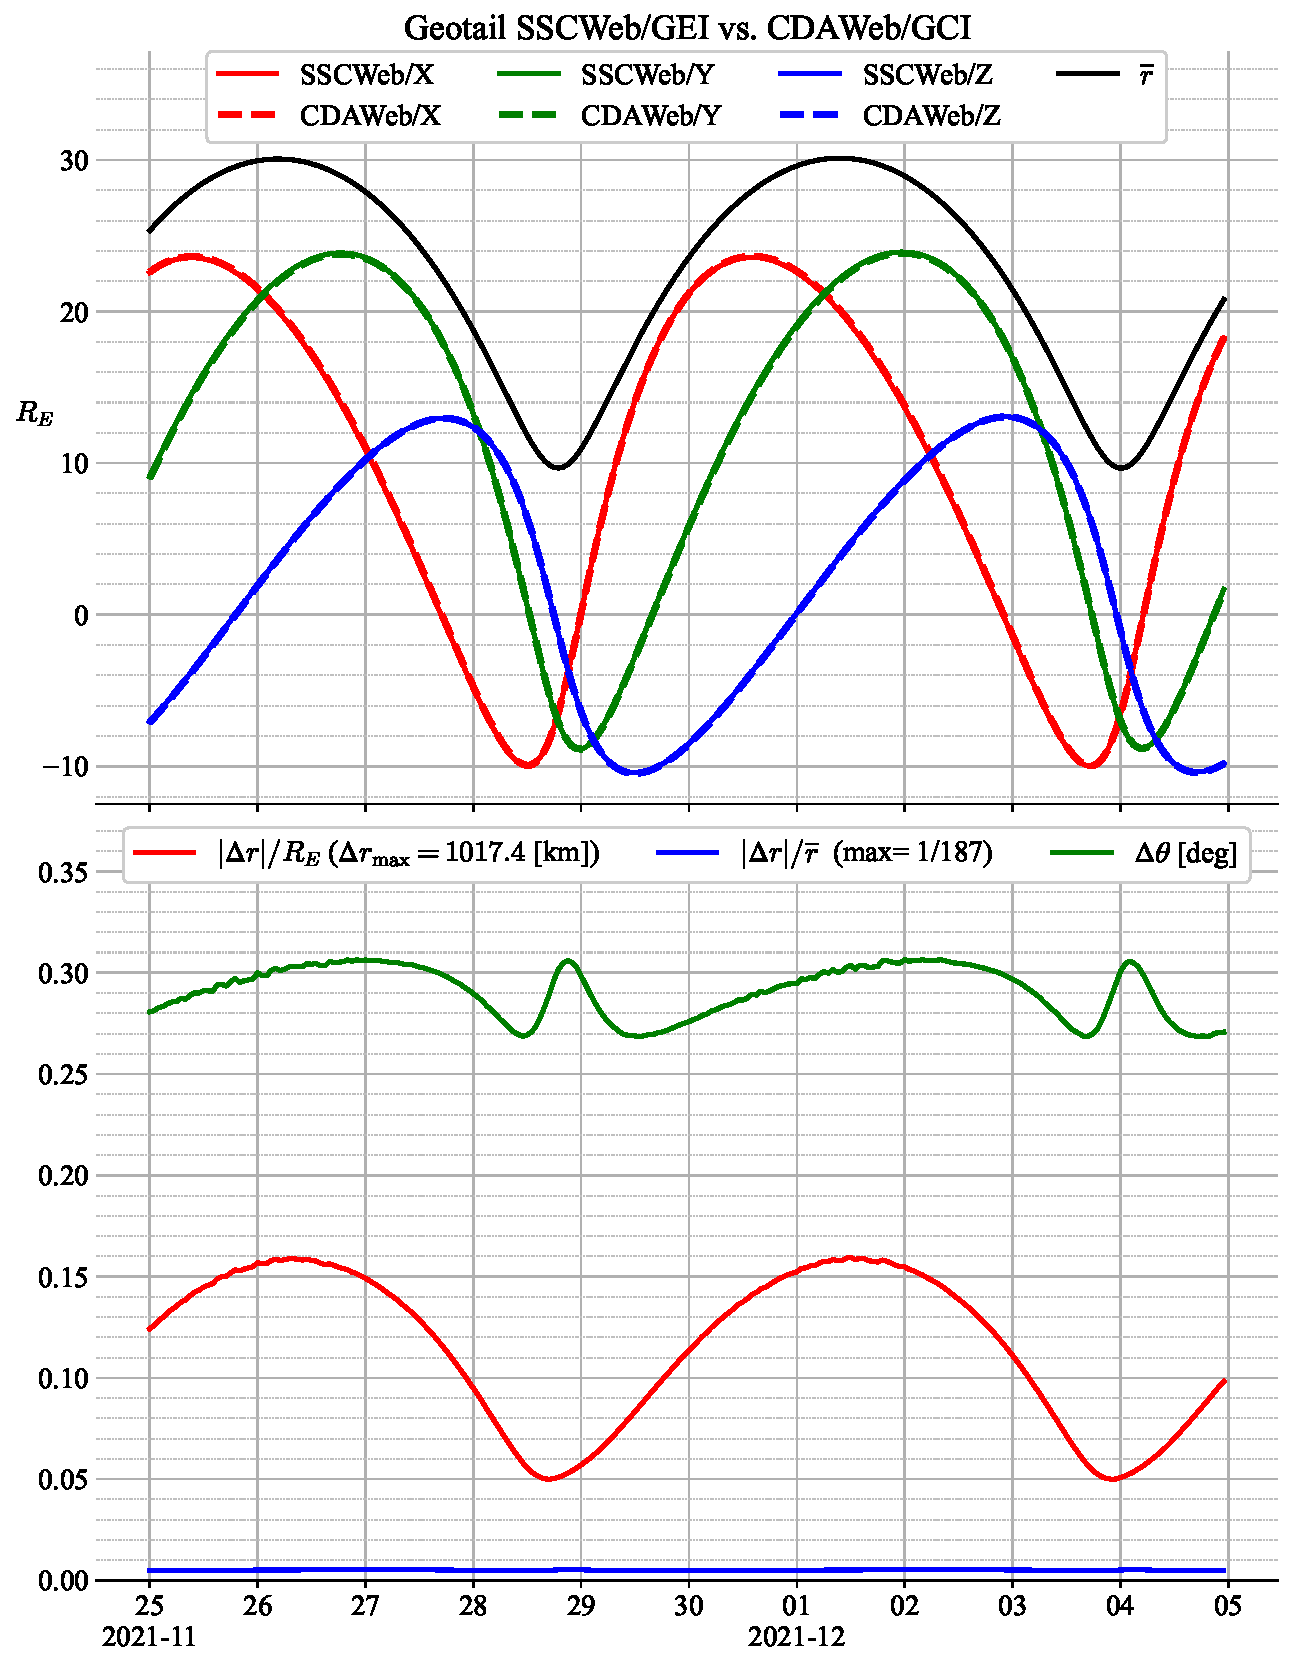
\includegraphics[width=\textwidth]{figures/Geotail_SSCWeb-GEI_vs_CDAWeb-GCI.pdf}
     \end{subfigure}
     \begin{subfigure}[b]{0.49\textwidth}
         (b)
         \centering
         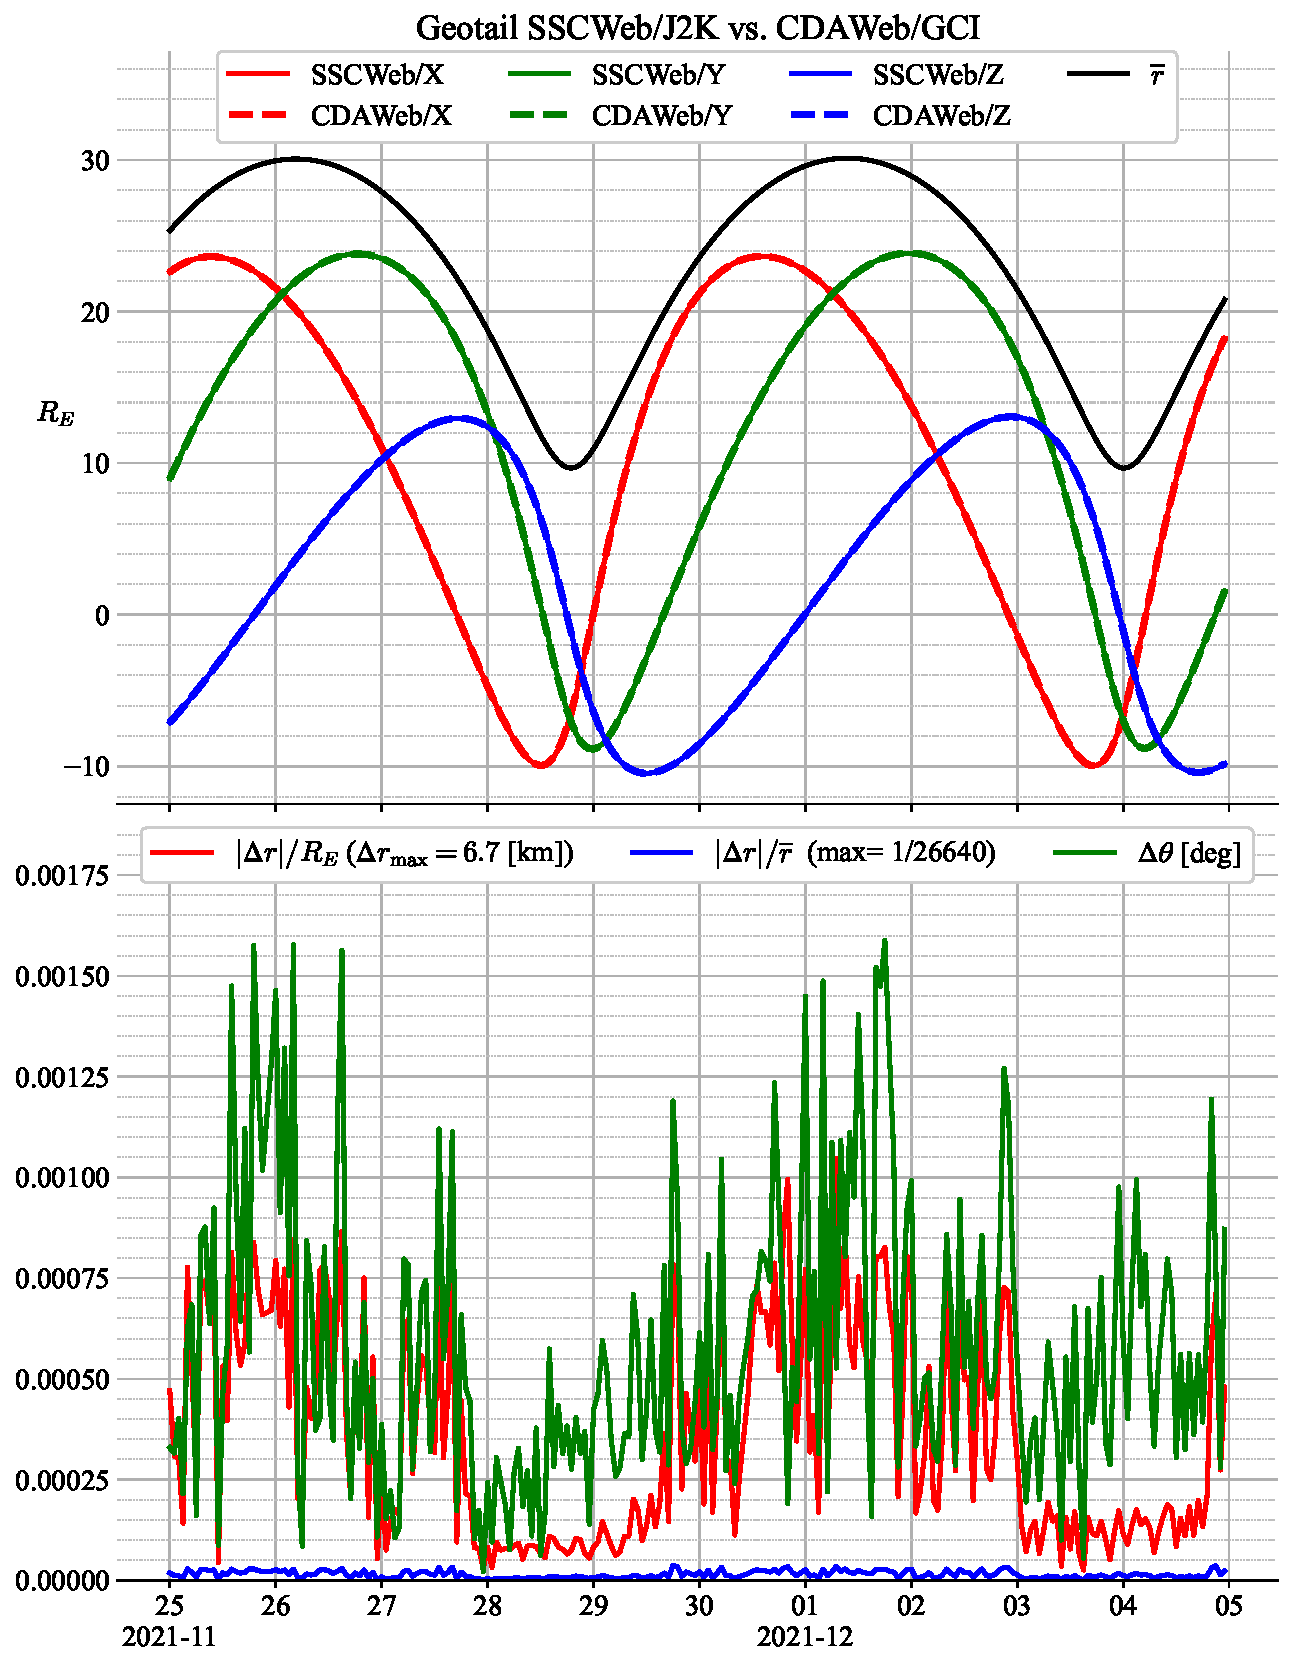
\includegraphics[width=\textwidth]{figures/Geotail_SSCWeb-J2K_vs_CDAWeb-GCI.pdf}
     \end{subfigure}
     \par\bigskip\bigskip
     \begin{subfigure}[b]{0.49\textwidth}
         (c)
         \centering
         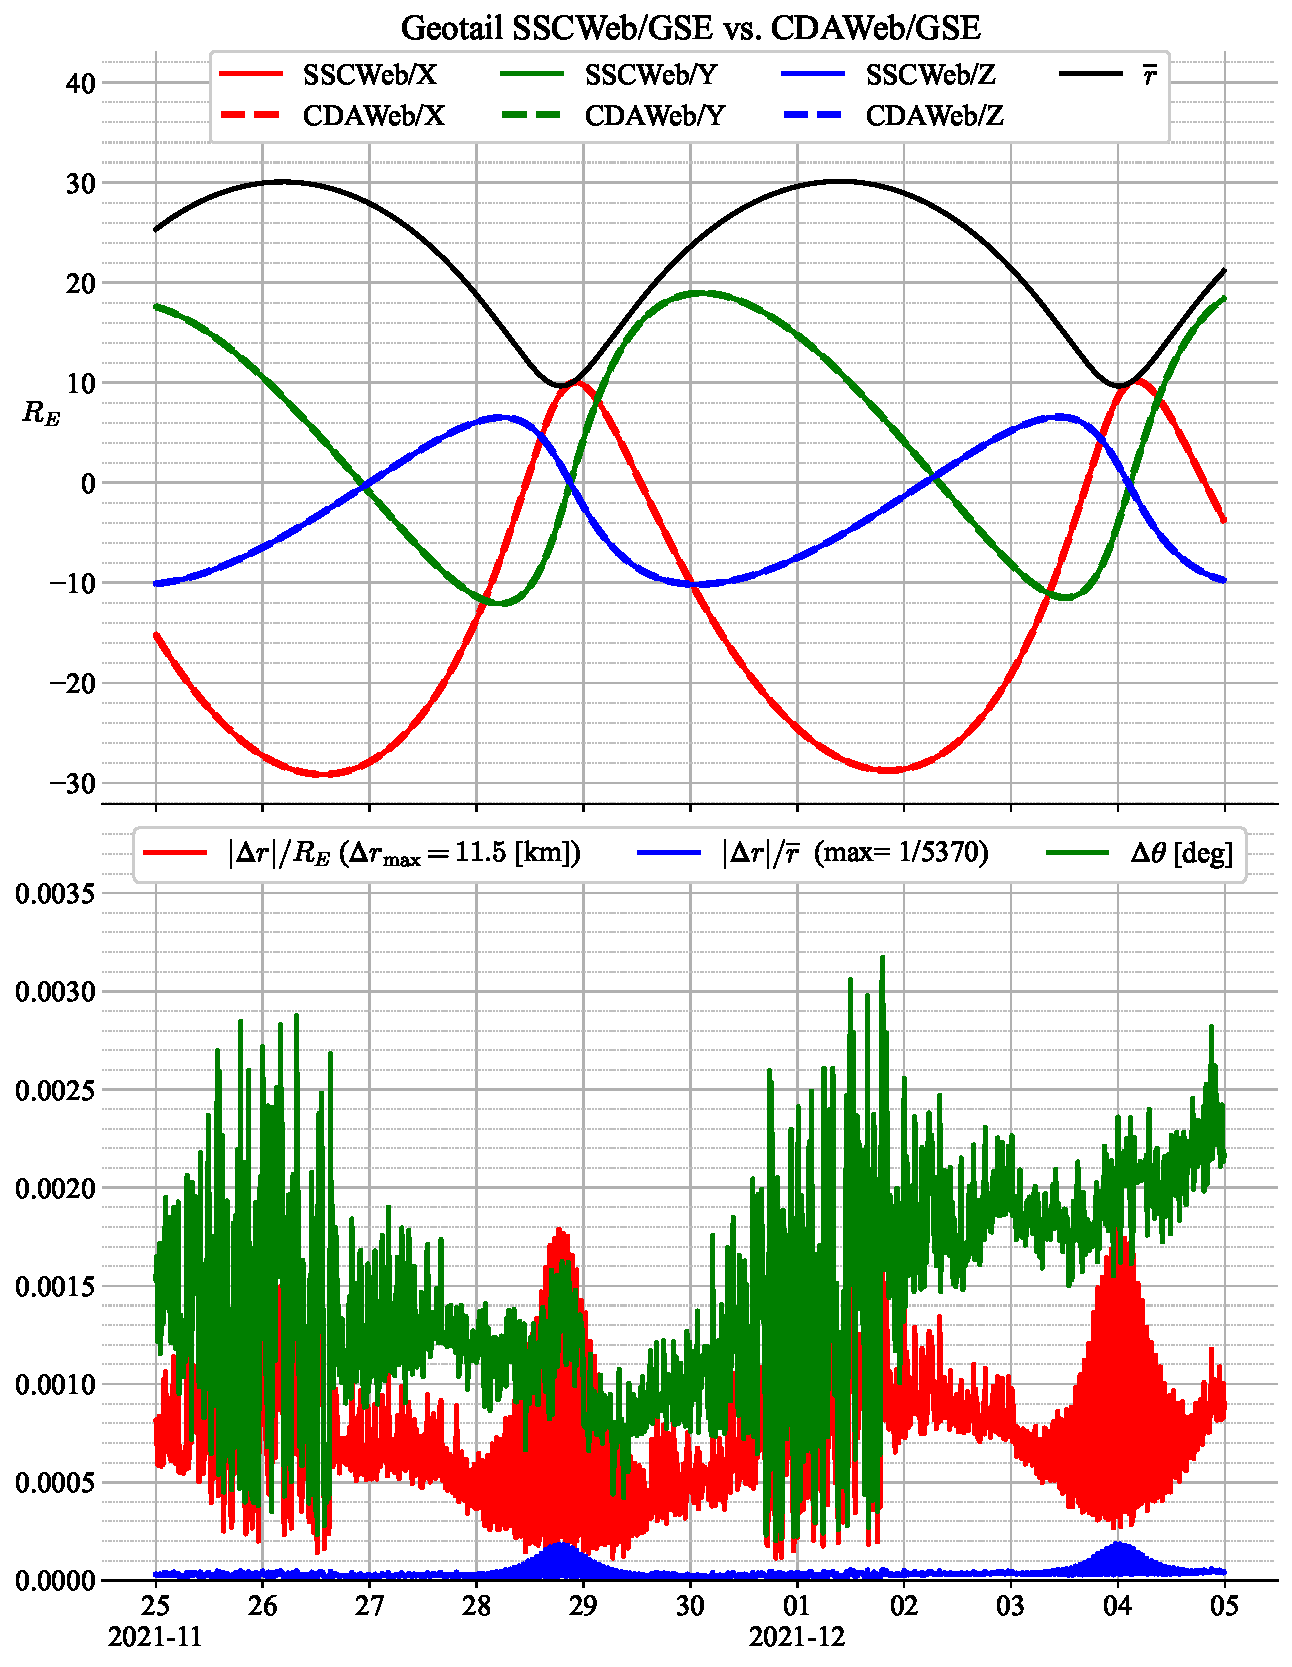
\includegraphics[width=\textwidth]{figures/Geotail_SSCWeb-GSE_vs_CDAWeb-GSE.pdf}
     \end{subfigure}
     \begin{subfigure}[b]{0.49\textwidth}
         (d)
         \centering
         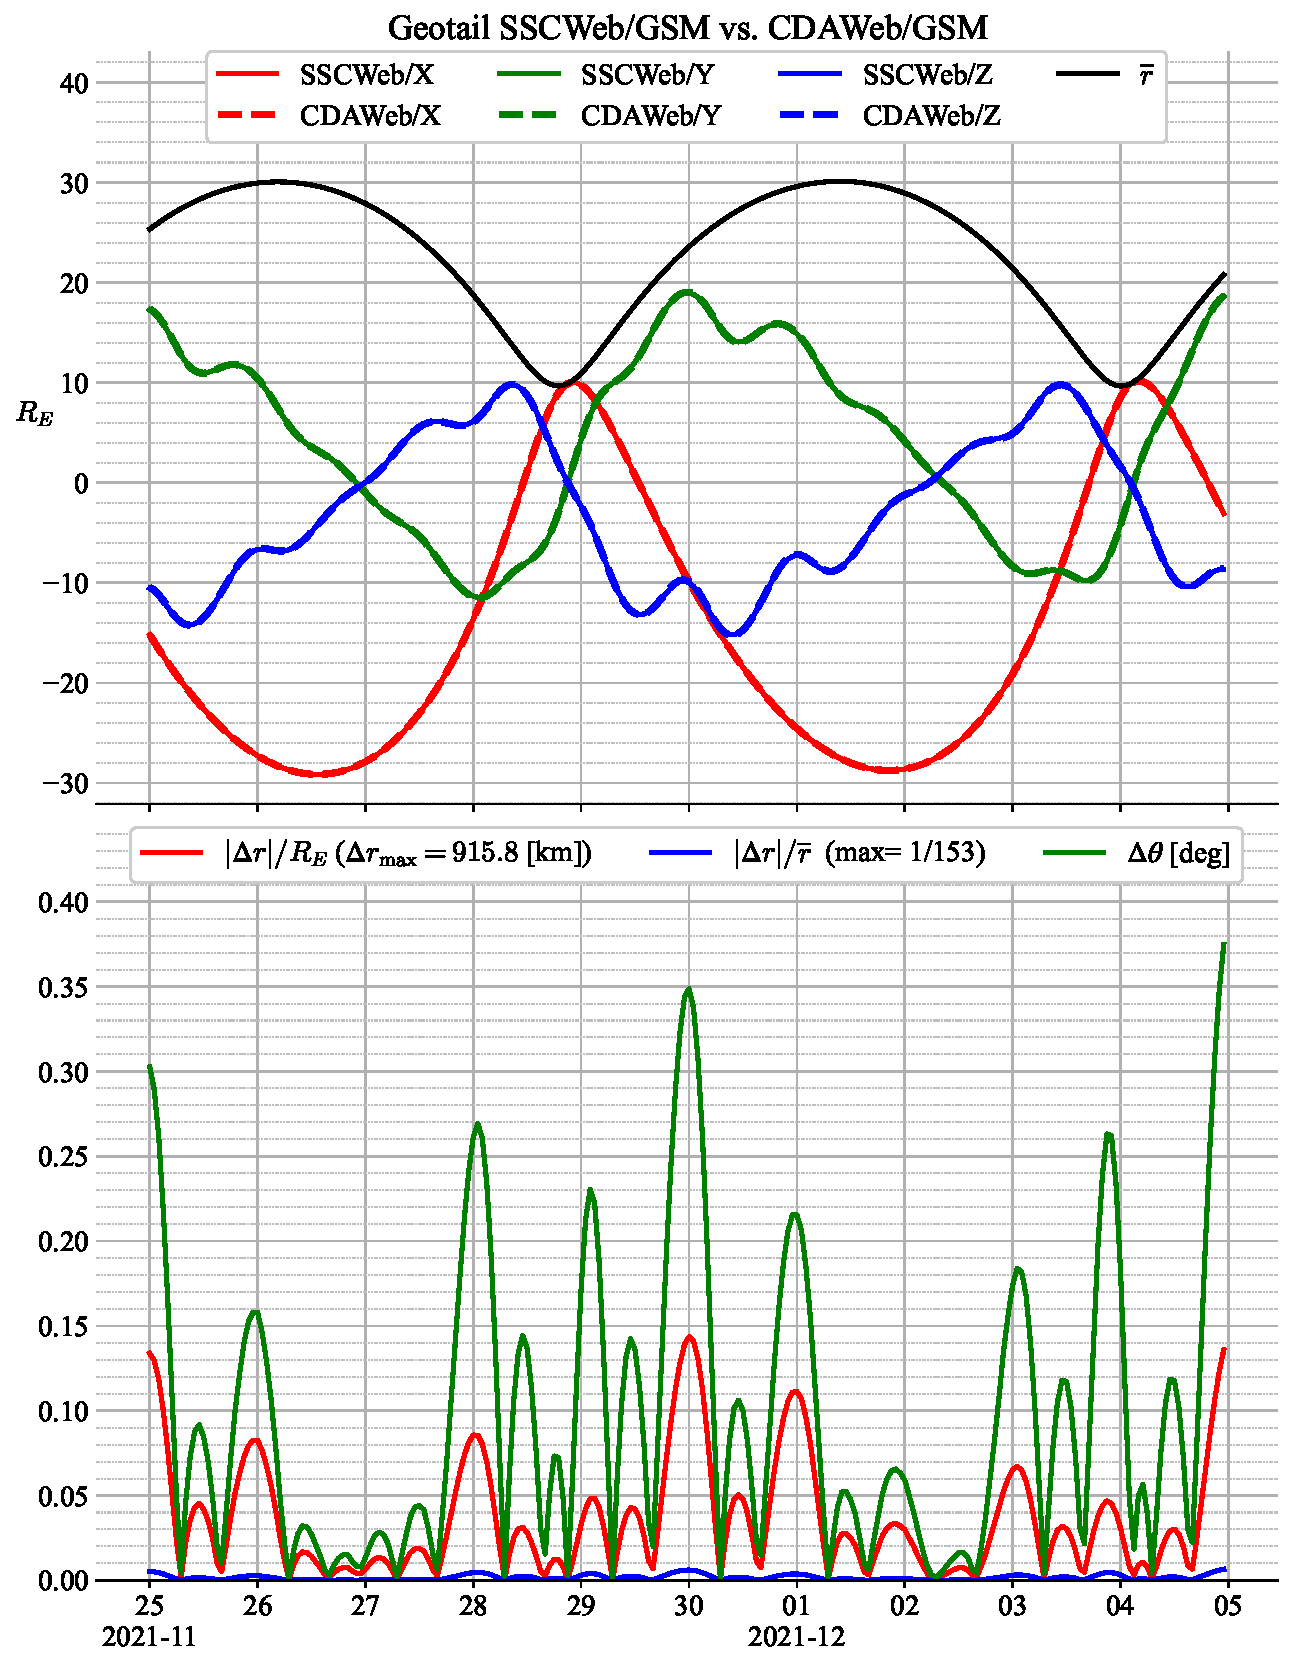
\includegraphics[width=\textwidth]{figures/Geotail_SSCWeb-GSM_vs_CDAWeb-GSM.pdf}
     \end{subfigure}
     \caption{Comparison of ephemeris values from SSCWeb and CDAWeb in four different reference systems.}
     \label{fig:geotail}
\end{figure}

\clearpage

\begin{figure}[h]
     \begin{subfigure}[b]{0.49\textwidth}
         (a)
         \centering
         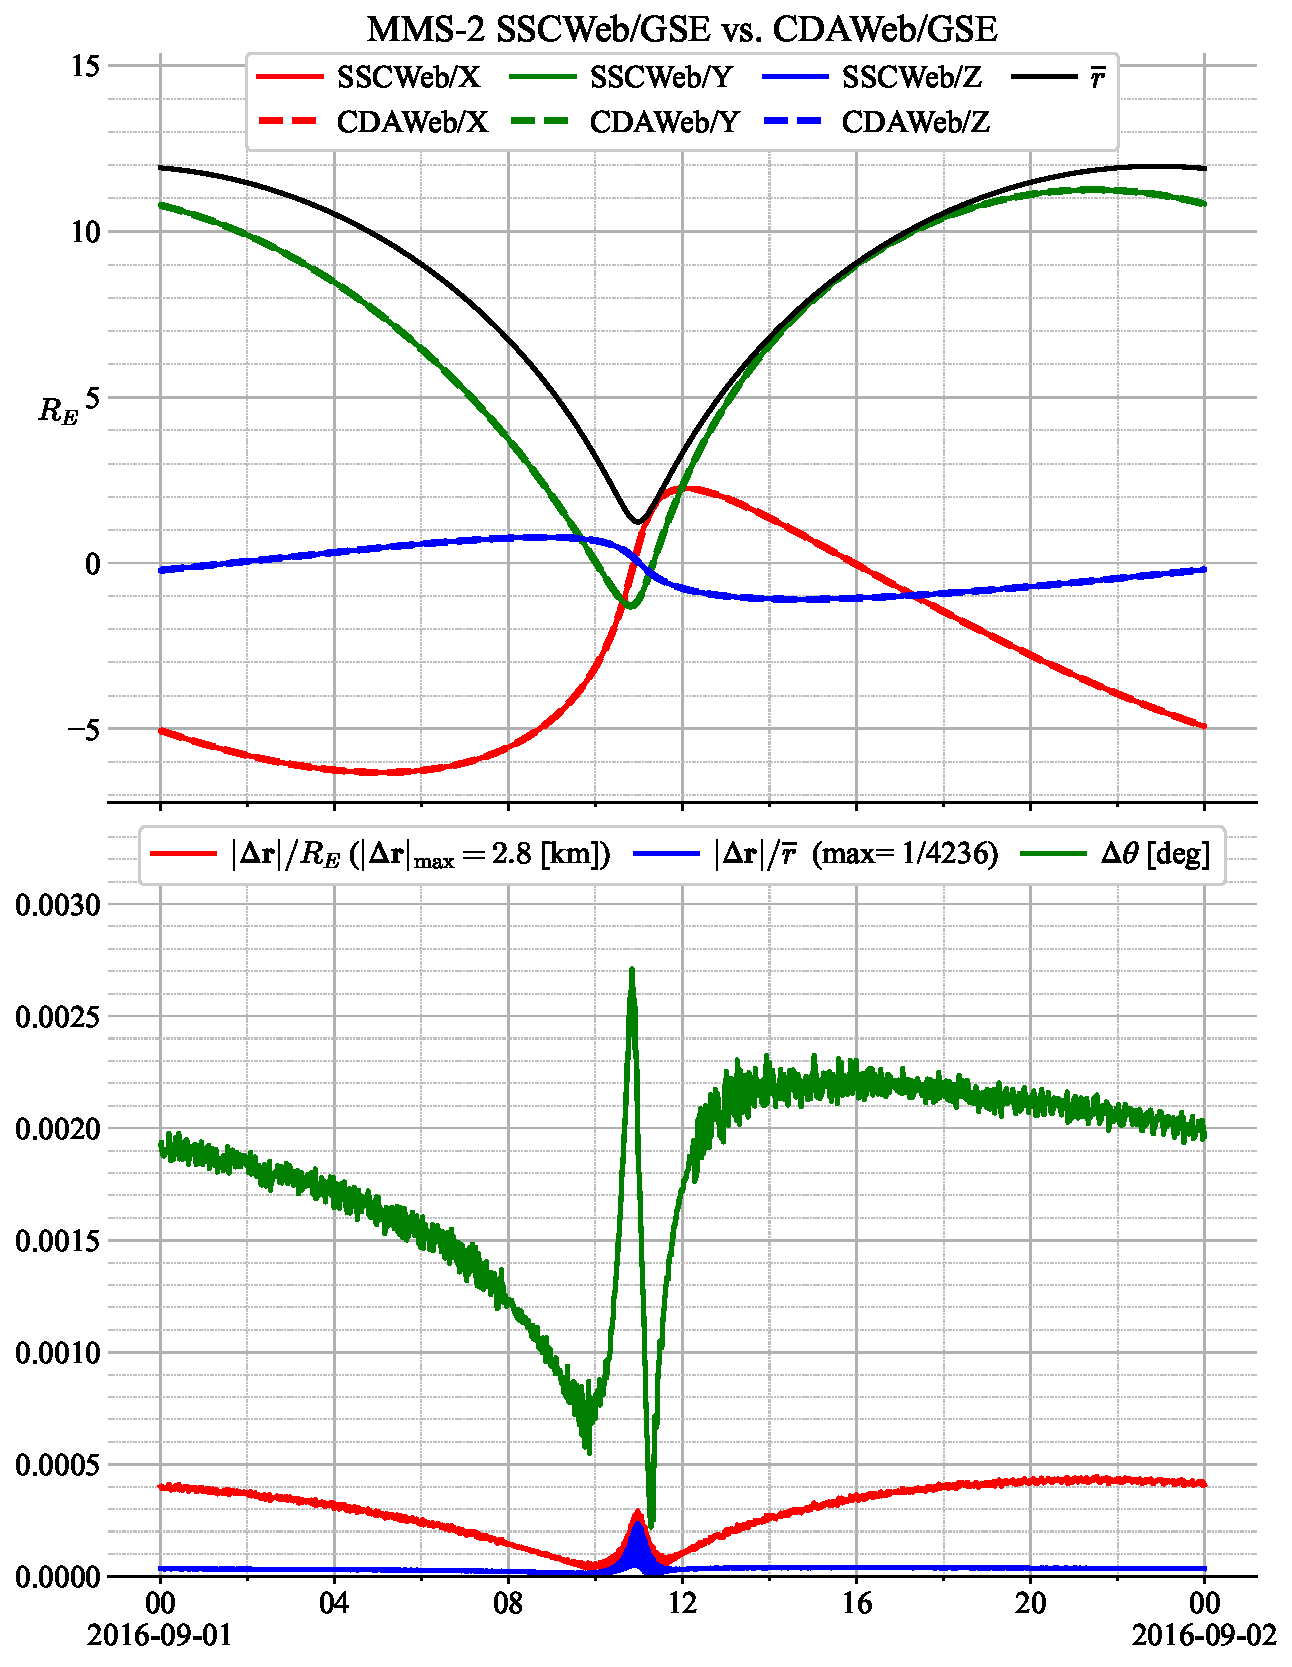
\includegraphics[width=\textwidth]{code/figures/ephemeris/MMS-2_SSCWeb-GSE_vs_CDAWeb-GSE.pdf}
     \end{subfigure}
     \begin{subfigure}[b]{0.49\textwidth}
         (b)
         \centering
         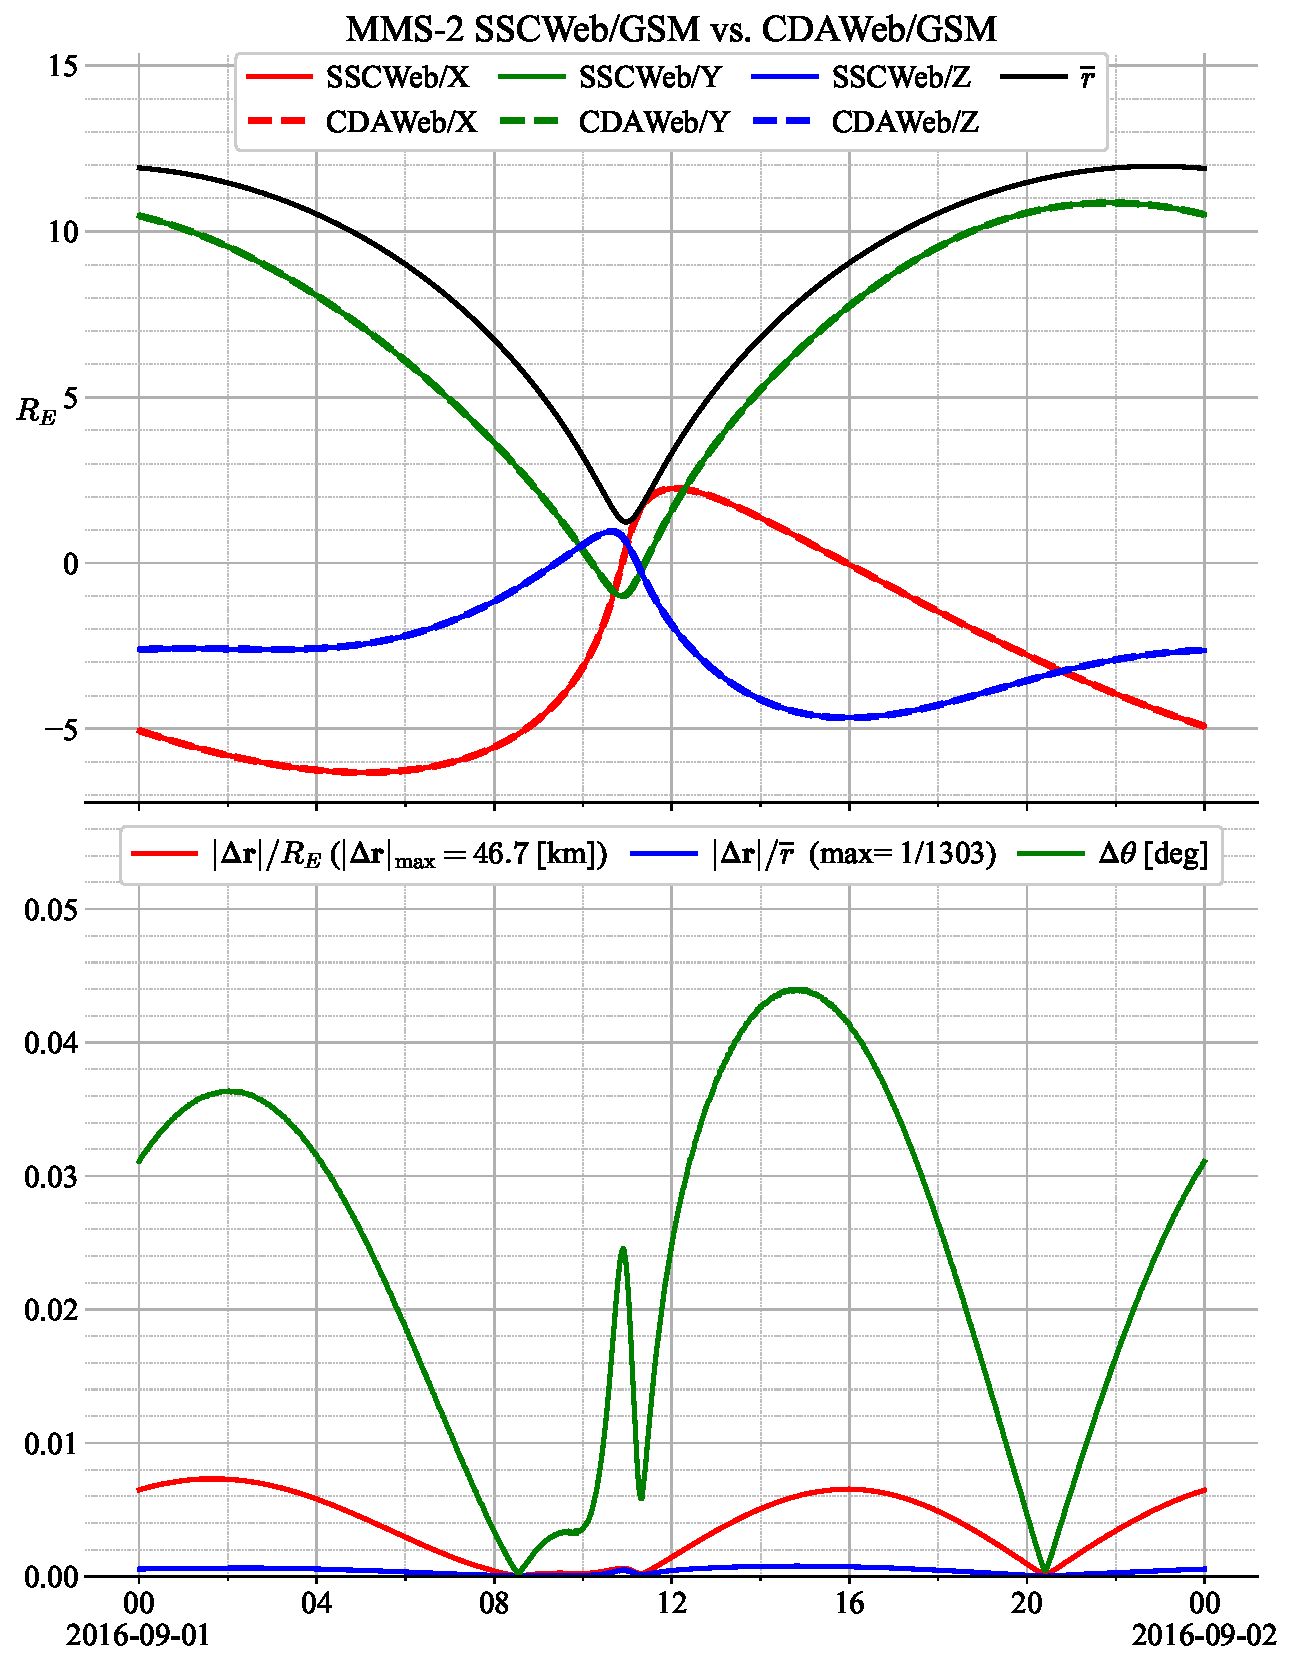
\includegraphics[width=\textwidth]{code/figures/ephemeris/MMS-2_SSCWeb-GSM_vs_CDAWeb-GSM.pdf}
     \end{subfigure}
     \par\bigskip\bigskip
     \begin{subfigure}[b]{0.49\textwidth}
         (c)
         \centering
         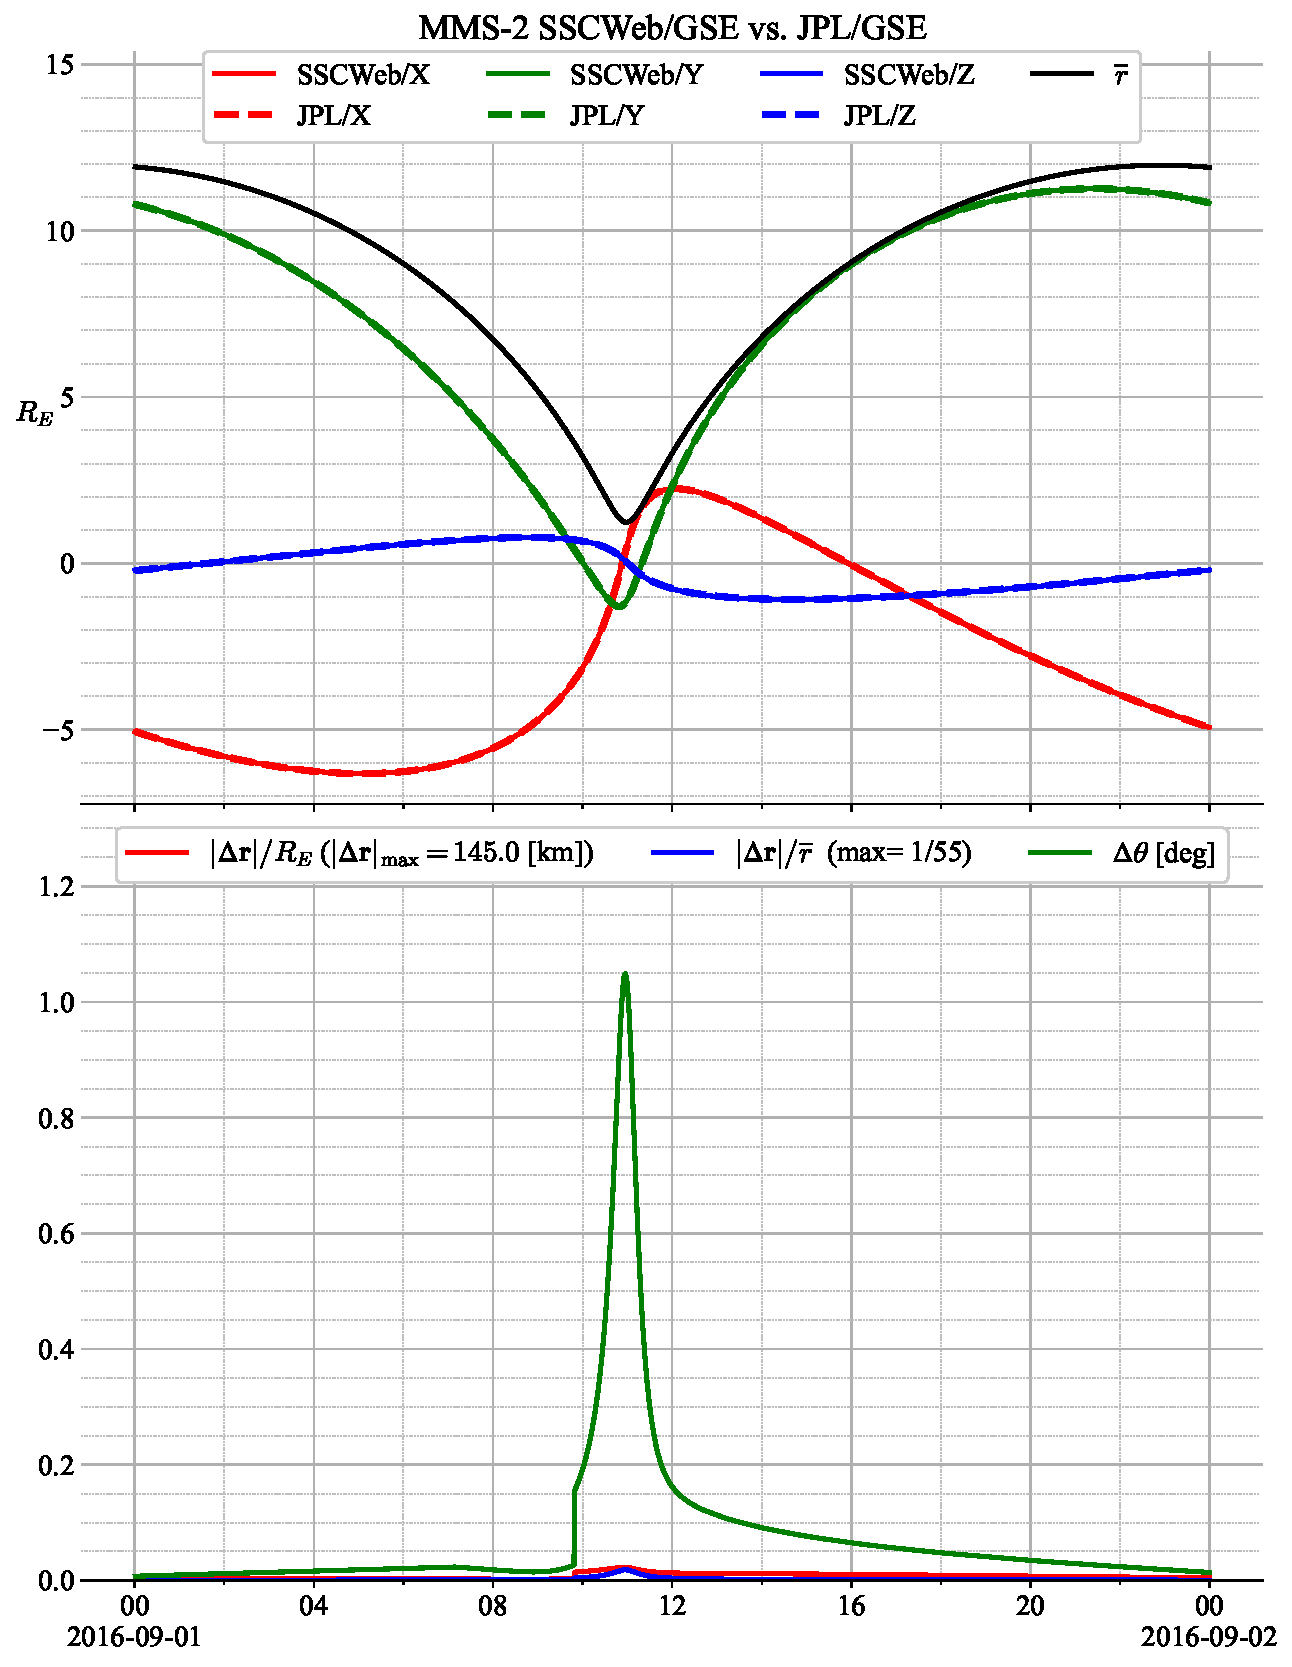
\includegraphics[width=\textwidth]{code/figures/ephemeris/MMS-2_SSCWeb-GSE_vs_JPL-GSE.pdf}
     \end{subfigure}
     \begin{subfigure}[b]{0.49\textwidth}
         (d)
         \centering
         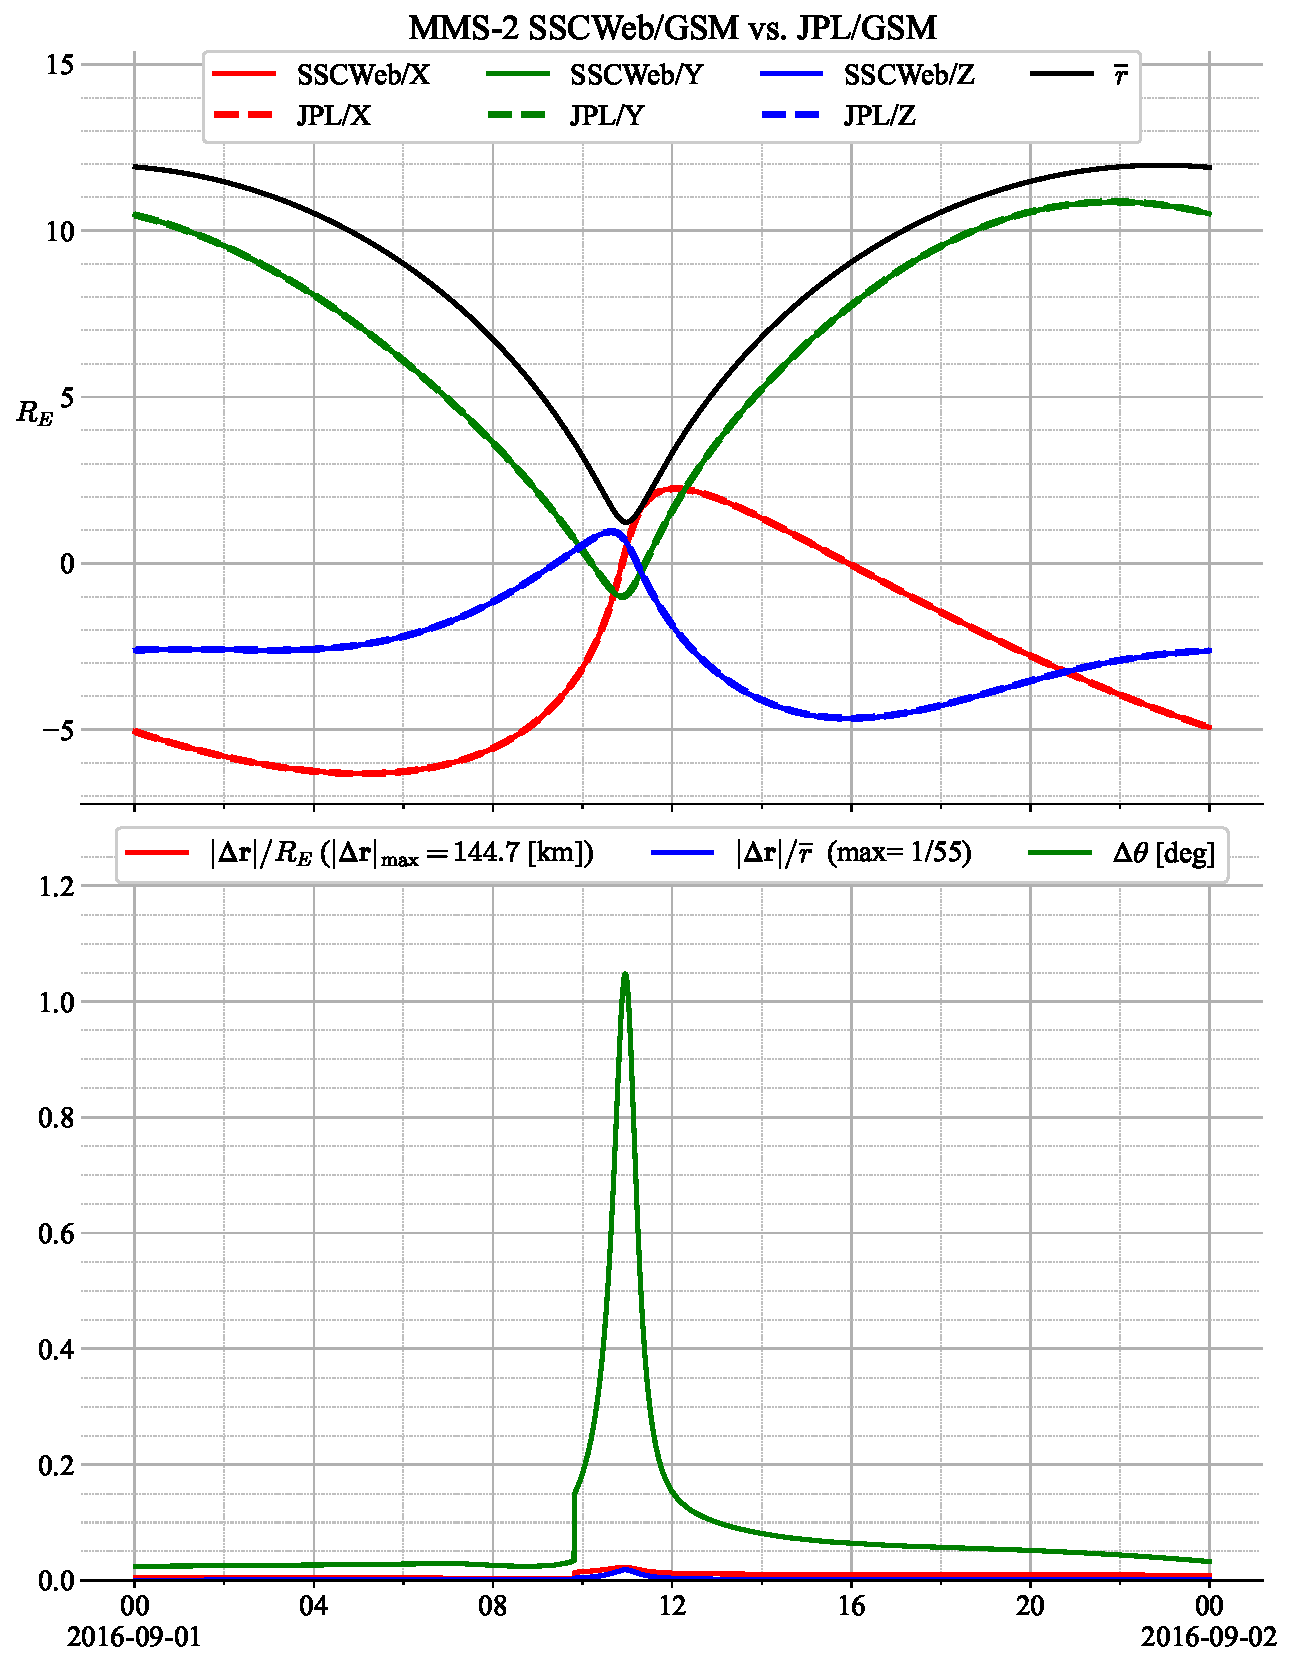
\includegraphics[width=\textwidth]{code/figures/ephemeris/MMS-2_SSCWeb-GSM_vs_JPL-GSM.pdf}
     \end{subfigure}
     \caption{}
     \label{fig:mms-2}
\end{figure}

\clearpage

%These calculations were based on ... ISTP software. The results from \citeA{SSCWeb} were obtained using its web interface, which dynamically computes results based on ...

%\todo[inline]{Finish after browsing code, which is private Google Drive folder 2023_STCT_NASA}.

%Another recommendation: service provides links to software used (sometimes not possible)

\subsection{Software}
\label{sect:comparisons_software}
\vspace{-1.5in}
\begin{figure}[htb]
     \begin{subfigure}[b]{0.49\textwidth}
         (a)
         \centering
         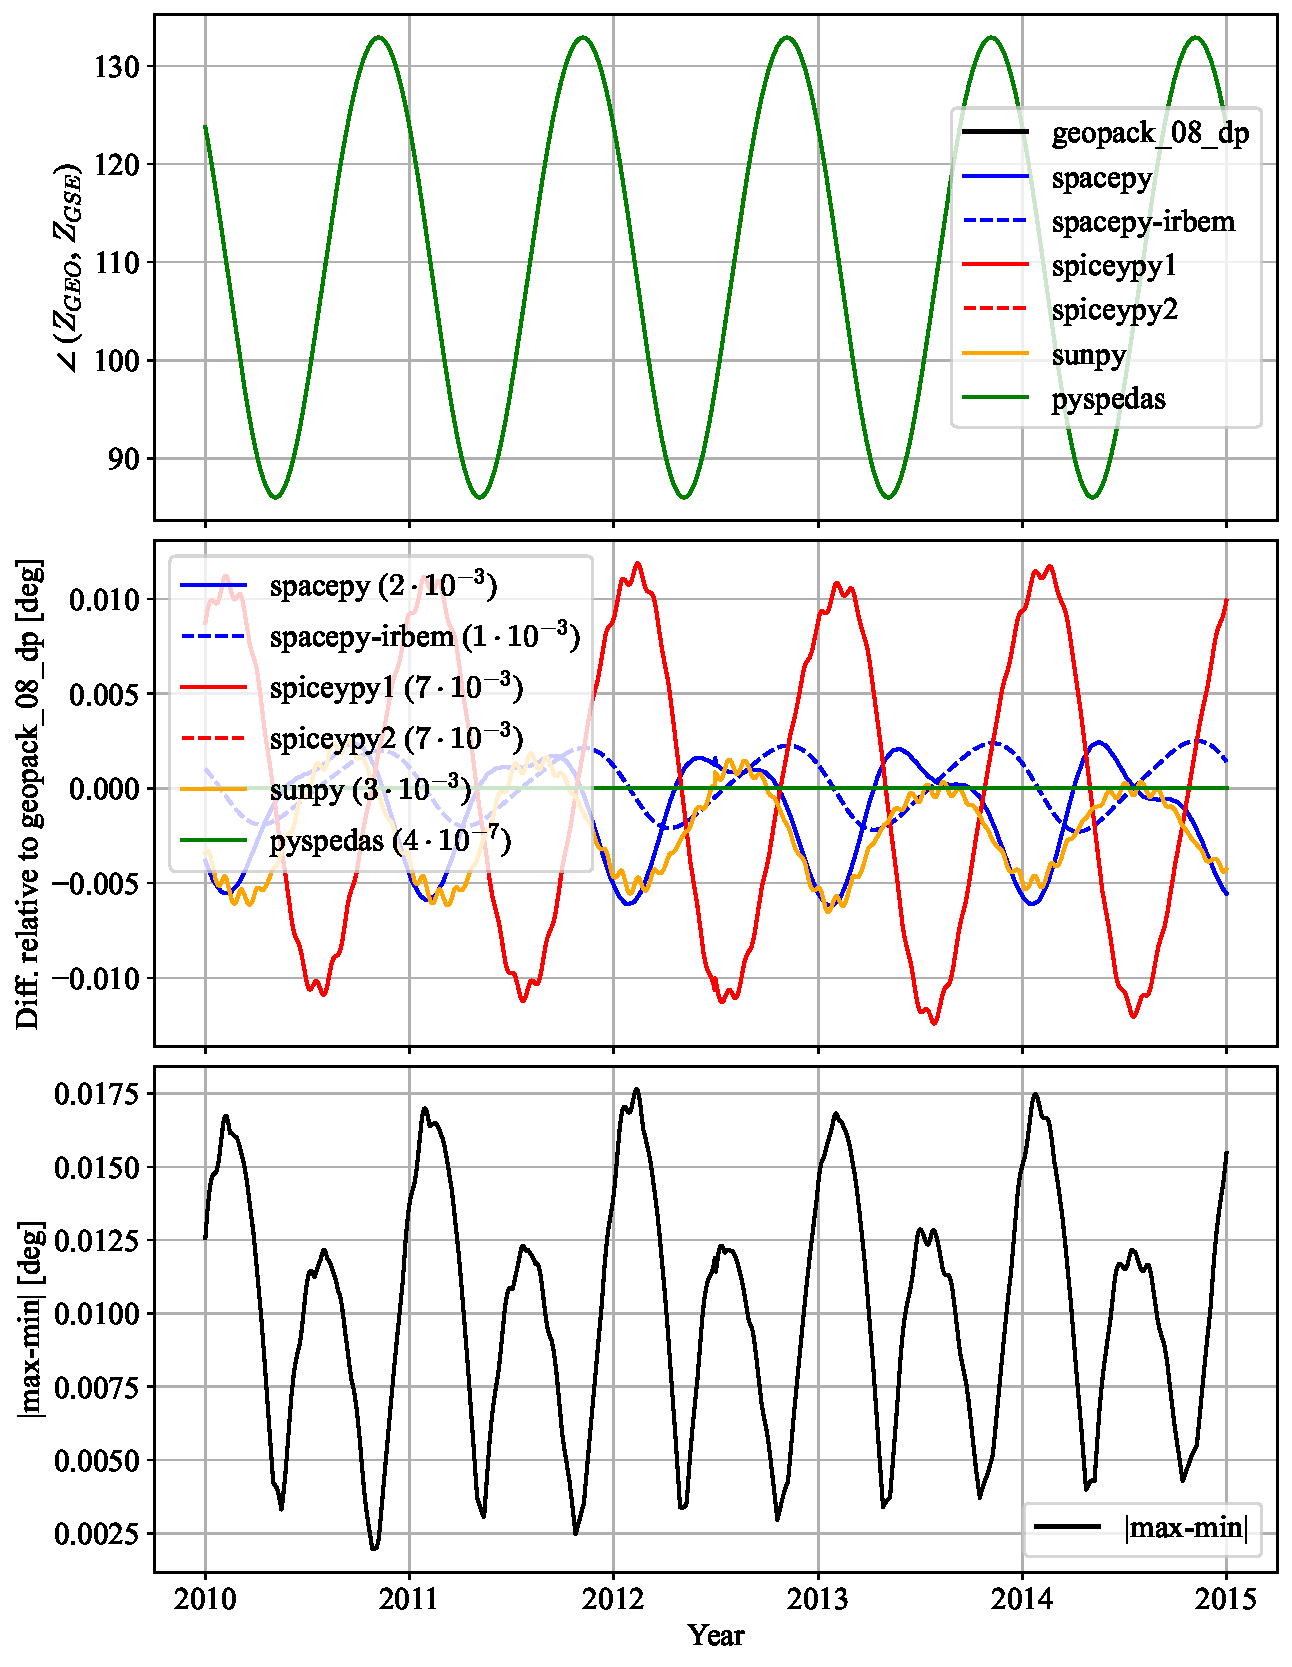
\includegraphics[width=\textwidth]{code/figures/angles/delta=1days_20100101-20150101/GEO_GSE.pdf}
     \end{subfigure}
     \begin{subfigure}[b]{0.49\textwidth}
         (b)
         \centering
         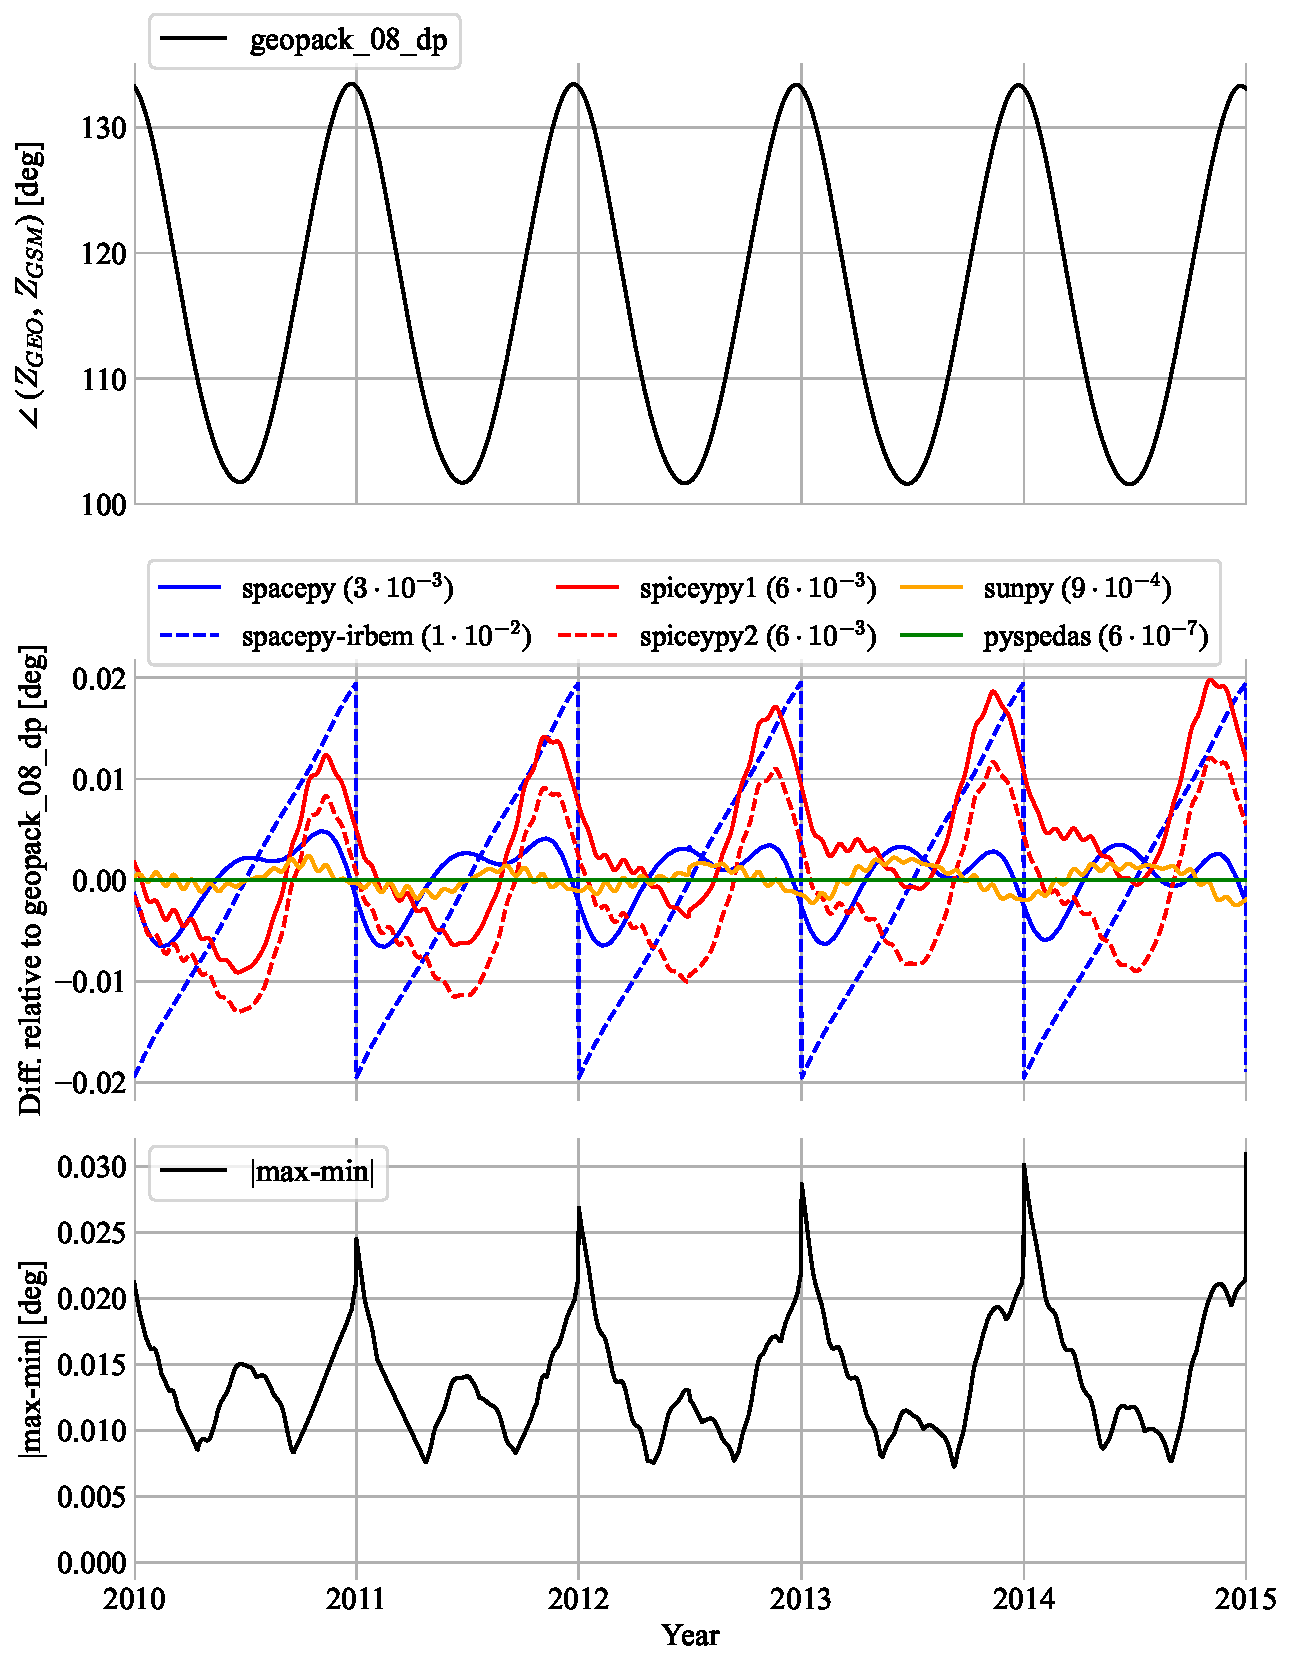
\includegraphics[width=\textwidth]{code/figures/angles/delta=1days_20100101-20150101/GEO_GSM.pdf}
     \end{subfigure}
     \par\bigskip\bigskip
     \begin{subfigure}[b]{0.49\textwidth}
         (c)
         \centering
         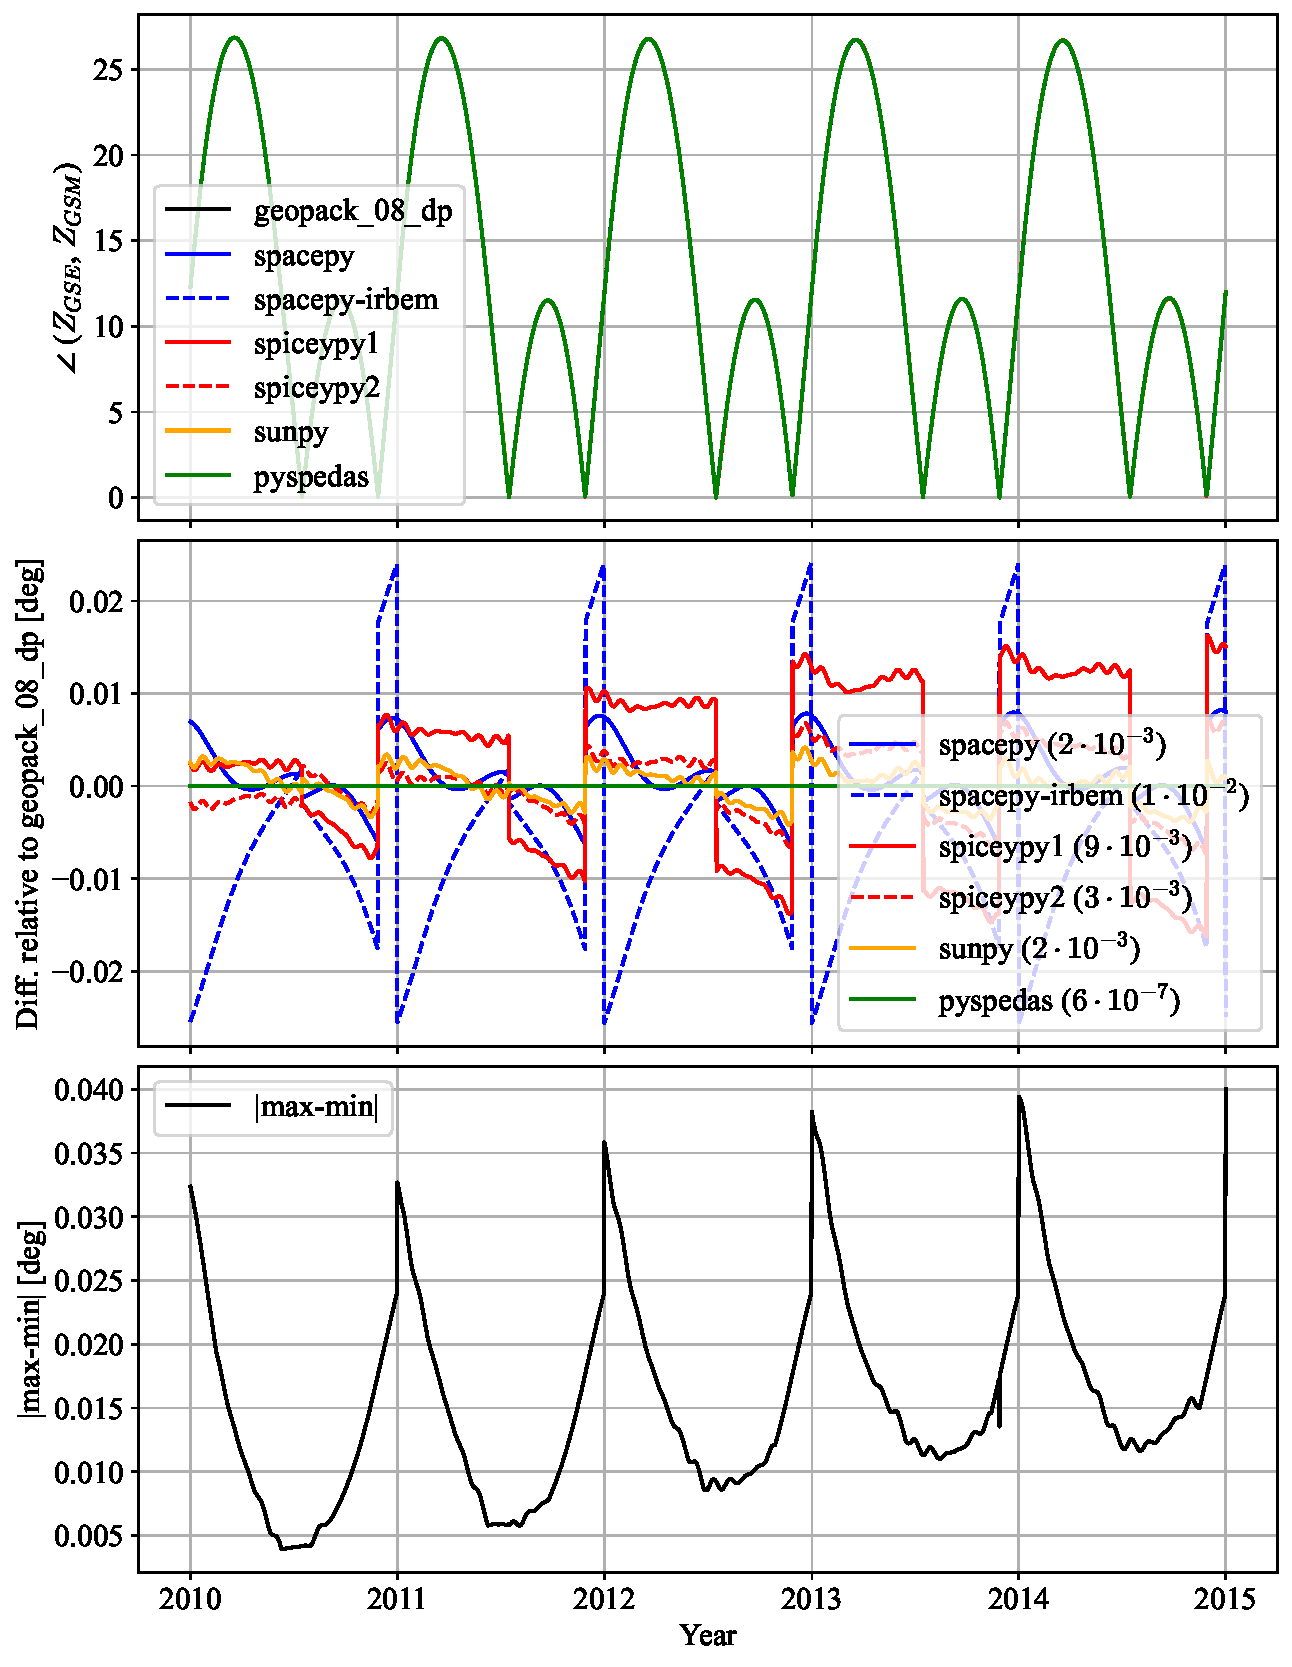
\includegraphics[width=\textwidth]{code/figures/angles/delta=1days_20100101-20150101/GSE_GSM.pdf}
     \end{subfigure}
     \begin{subfigure}[b]{0.49\textwidth}
         (d)
         \centering
         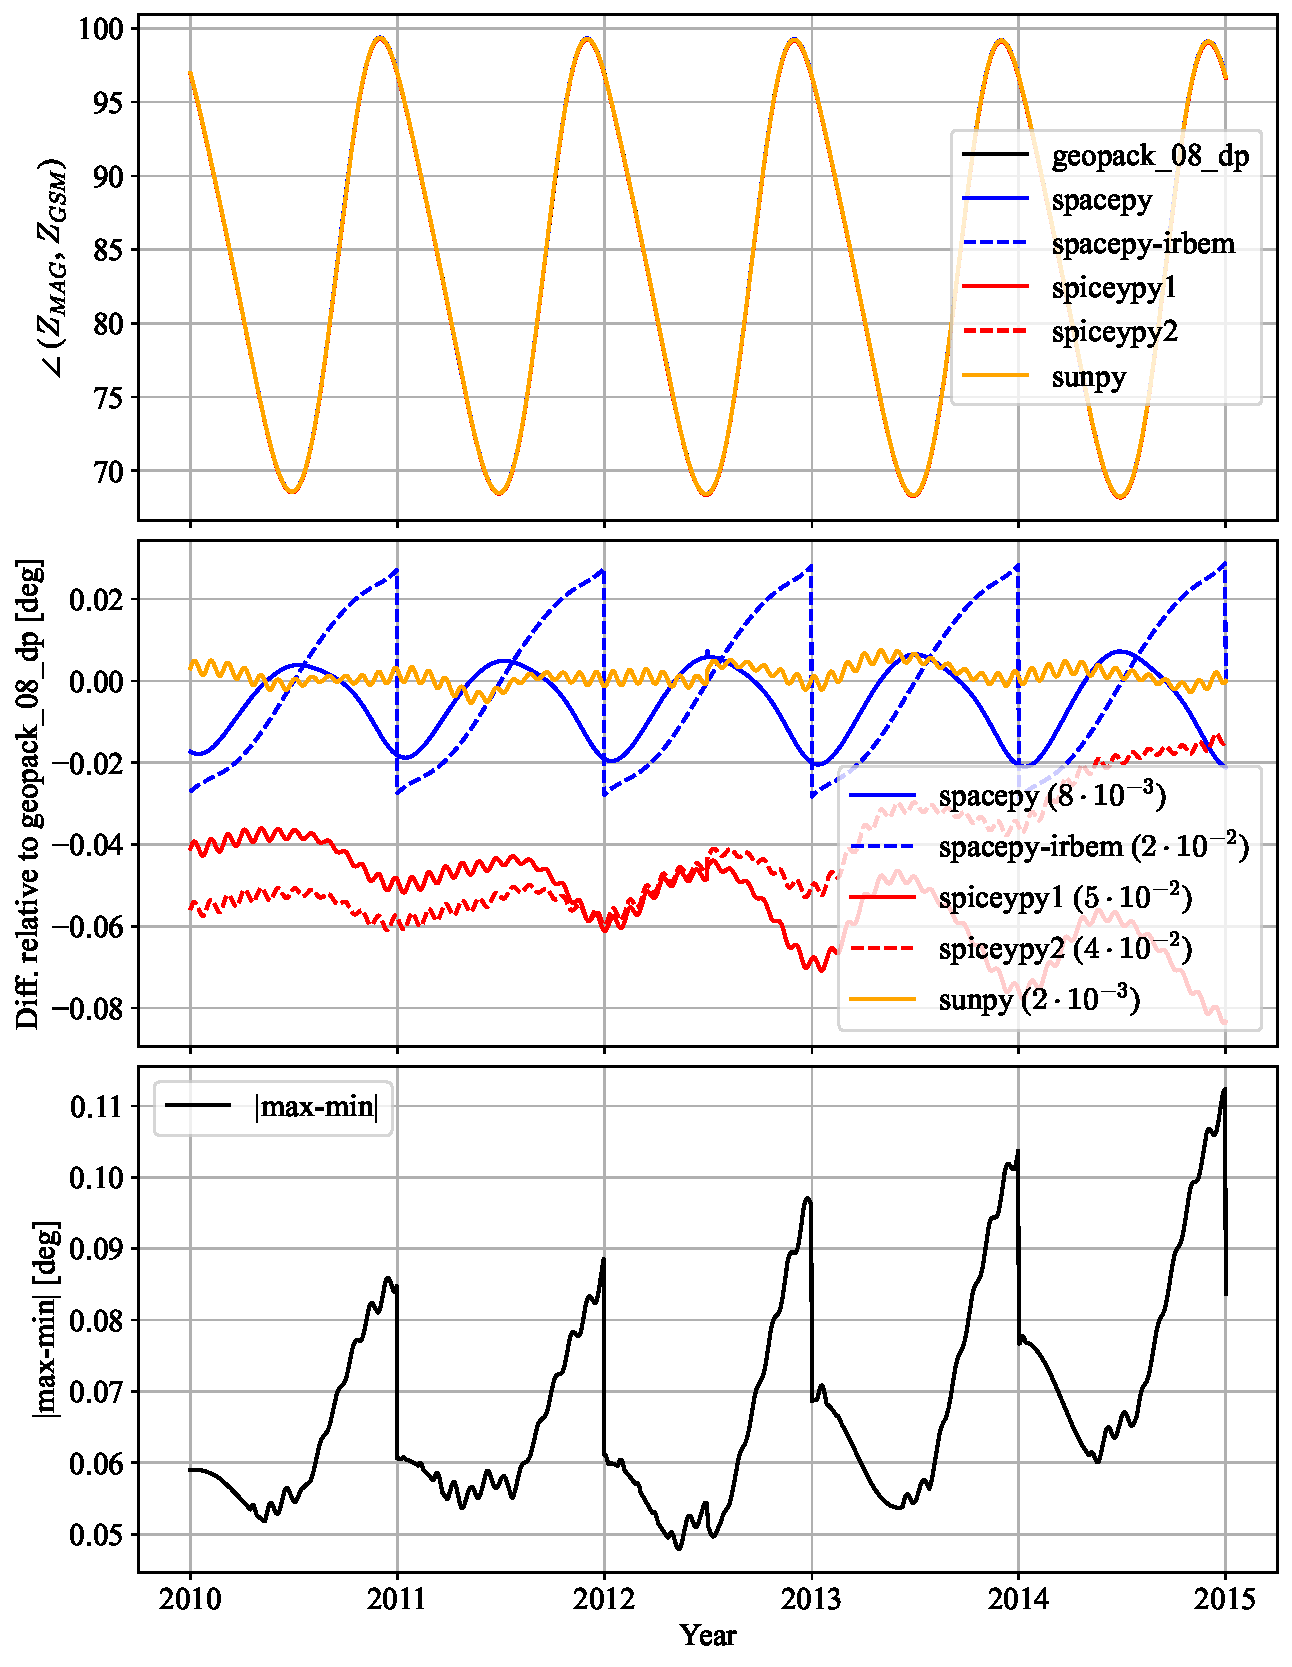
\includegraphics[width=\textwidth]{code/figures/angles/delta=1days_20100101-20150101/MAG_GSM.pdf}
     \end{subfigure}
     \caption{}
     \label{fig:angles}
\end{figure}

\clearpage

\small
\begin{verbatim}
Time: [2015, 12, 30, 0, 0, 0]
                           x           y           z       magnitude
-----------------------------------------------------------------------------------
Input (GSE):           3.46410162  3.46410162  3.46410162  6.00000000
Output (GSM):                                                         ang. [°]
                                                                      wrt Input
-----------------------------------------------------------------------------------
cxform                 3.46410162  2.54340625  4.18701381  6.00000000 11.19612022
geopack_08_dp          3.46410162  2.54785114  4.18431052  6.00000000 11.14656002
pyspedas               3.46410162  2.54785080  4.18431073  6.00000000 11.14656386
spacepy                3.46410162  2.54710195  4.18476662  6.00000000 11.15491581
spacepy-irbem          3.46410162  2.54566083  4.18535391  5.99979803 11.16945855
spiceypy1              3.46410162  2.54651712  4.18512252  6.00000000 11.16143772
spiceypy2              3.46410162  2.54725501  4.18467345  6.00000000 11.15320876
sscweb                 3.46        2.55        4.18        5.99554001 11.10894044
sunpy                  3.46395412  2.54785162  4.18443234  6.00000000 11.14727882

max-min:               0.00410162  0.00659375  0.00701381  0.00445999  0.08717978
100*|max-min|/|max|:       0.1184%     0.2586%     0.1675%     0.0743%     0.7787%
\end{verbatim}
\normalsize

\noindent
If $x$, $y$, $z$ are in $R_E$, then the $\mbox{max}-\mbox{min}$ angle corresponds to 58 km.

\section{How spacecraft missions develop transforms}
\label{sect:missions}

Data for space physics satellite missions typically include vector measurements in multiple coordinate systems. For \citeA{SSCWebProvenance}, three approaches have been taken:

\begin{enumerate}
    \parskip 0.1in 

    \item the mission develops SPICE kernels for ephemeris, and these kernels are ingested. The \texttt{GEI}--related SPICE kernel information is used to generate the \texttt{J2000} ephemeris.

    Delivery of SPICE kernels (if used) is not required by missions, so if a SPICE kernel is not available,

    \item A \texttt{GEI}--related variable in CDF files ingested from the mission database is used.

    \item TLE (two--line element) files are obtained from NORAD* and the a c translation of the NORAD SGP4 Pascal Library \cite{NORADSGP4c} is used to compute ephemeris in \texttt{TEME} Then, ISTP--era software is used to compute ephemeris in different coordinate systems. The ISTP software uses proprietary information needed for the transforms (sun position) calculated by GSFC's Flight Dynamic Facility, FDF. If an existing SPICE kernel has coordinate transform information, it is not used and if the CDF files have ephemeris in different coordinate systems, they are not used.

    % Hoots and Roehrich [1988]: ``The most important point to be noted is that not just any prediction model will suffice. The NORAD element sets are ``mean" values obtained by removing periodic variations in a particular way. In order to obtain good predictions, these periodic variations must be reconstructed (by the prediction model) in exactly the same way they were removed by NORAD." Hence the NORAD SGP4 and SDP4 orbit predictor models give the best orbit predictions using TLEs. Felix R., Hoots, F. R., R. L. Roehrich, SPACETRACK REPORT NO. 3 Models for Propagation of NORAD Element Sets, December 1 980 Package Compiled by TS Kelso 31 December 1988.
\end{enumerate}

* (special arrangement regarding military s/c),
Albert: ESA defined \texttt{HEE} differently from NASA in Solar Orbiter SPICE kernel see \texttt{SOLO\_HEE\_NASA} and \texttt{SOLO\_HEE} in \url{https://spiftp.esac.esa.int/data/SPICE/SOLAR-ORBITER/kernels/fk/solo_ANC_soc-sci-fk_V02.tf}

%TLEs are from CelesTrek and can't be distributed. Are public TLE repos, but are they the same?

%Discuss fact that TLEs, location info provenance may never be available, but should be aware of how it is done.

% Need to recommend ISTP name convention for GEI_2000 varaibles in CDF files. Getting agreement on names not possible, but could use attribute.

%https://sscweb.gsfc.nasa.gov/sscweb_data_provenance.html the SPICE kernels are obtained by ingest of directories. "Would be nice if required data delivery was SPICE kernels instead of being ancillary". In some cases, missions does provide SPICE kernels, in which case they use TLEs. TLEs less accurate than SPICE kernels and can't to predict as far out as in SPICE (which can use full time history).

%Ivar: given spk file with positions in gei_2000. How they did transforms to get there is not documented ... (e.g., from gps to gei_2000). Ivar gets csv values from Millenum xyz, vx, vy, vz (state information).

Tracers location is determined by GPS from Millenium space systems (running moc) then they compute GPS to GEI (use GEI_2000) and deliver to mission.

\section{Conclusions and Recommendations}
\label{sect:conclusions}

Comment on definition of $R_E$ and problem with providing measurements in terms of $R_E$.

In this section, we provide three recommendations to address the problems identified in this paper. No single recommendation will address all of the problems or satisfy all of the use cases.

\subsection{Database of transforms}

We note that for a given transform, all methods need to compute the same quantity: a transformation matrix at an instant in time. We also note that implementation of transforms requires technical expertise in software and also maintenance (for example, updating IGRF coefficients). Based on this, we recommend that a reference dataset is developed (and kept up-to-date). Each record in the dataset will be a timestamp and a matrix that is required to transform from a given coordinate system to a reference coordinate system. The records should be at 1--second cadence or less and be made available in CDF files.

With such a dataset, if a scientist wants to allow for reproducibility, they could state ``the vector measurements in \textttt{ABC} were transformed into coordinate system \textttt{XYZ}," by using \textttt{ABC} to \textttt{REF} and \textttt{REF} to \textttt{XYZ} transformation matrices in the reference dataset.

We have found that many software libraries do spot checks of transforms. For example, SunPy's unit tests \cite{SunPy} compares with table from \citeA{Franz2002} at one time instant. \cite{cxform} compares with \citeA{SSCWeb} results (which only provide answers to two decimal places). With the proposed database, a software library developer could provide a comprehensive comparison with the reference dataset, which would allow users to be able to estimate uncertainties associated with coordinate transforms.

We also suggest that this dataset contains common time representations. Each record should be a UTC timestamp along with values for \texttt{CDF\_EPOCH}, \texttt{CDF\_TT2000}, \texttt{TAI}, etc. Although these time relationships are much easier to compute, some require leap second tables and to perform the computation, one needs to parse (and update if needed) the leap second table. An additional advantage of this dataset is that software developers can use it for unit testing their own implementations.

As demonstrated in Section~\ref{sect:comparisons}, differences exist. Debugging and understanding how code works is difficult.

Issues with updates of IGRF, for example.

Not all users will prefer to use a dataset for transformation.

This database may not be usable for all applications. However, it can still be used as a reference. For example, suppose the dataset provides transforms at 1--second cadence, but software generates transforms at a millisecond cadence (and interpolation is not acceptable). The software provider can validate their transforms and make a statement such as ``the transforms match the reference dataset to a precision of … at the 1--minute values provided by the reference dataset".

One advantage of this dataset in comparison to the use of software libraries is that software libraries require continual upgrades and having software automatically updating IGRF coefficients and leap second information may work at present, not all software will be maintained indefinitely into the future. In addition, transform results may change as a given software package evolves. As an example, consider a package that uses preliminary IGRF for MAG and computes a transform. Five years later, the result will not be the same if the the software now uses definitive IGRF coefficients. Although it is possible in principle for the package developers to maintain reproducibility, doing so requires significant effort. The proposed dataset could address this by having two MAG coordinate systems. One uses only definitive IGRF coefficients. The other only uses non--definitive.

\subsection{Database of SPICE kernels}

Motivation: They are difficult to develop. For example, computing MAG transform requires a polynomial estimate of ...

\todo[inline]{Someone noted: SPICE kernel - ephemeris vs frame kernels; some don't want to share exact orbit for security reasons.}

\todo[inline]{
Ask Scott where Kernels are stored talk to planetrary folks. Post to Zenodo and use keyword SPICE + ???
}

\todo[inline]{
Interest from NASA for making modular … reason for Science Data Workshop.
}

Central location for SPICE kernels (how does planetary do it?) Use Zenodo or NAIF?

MAG example - if reference kernel was available, would need to be well documented (derivation, uncertainties, caveats, limitations). If someone wants to use a different kernel, they would be expected to compare their results with reference and justify reason why their definition is better given it will make replicability/comparison difficult.

Development/iteration approach. Plot comparison of different implementations. Will help end user who would need to do this.

PDS has tag with metakernel.

Issue with IGRF vs Chaos model.

Path forward - committee of former instrument people.

% Recommendation for Re: SpacePy = 6378.137km; IRBEM = 6371.2 km; SSCWeb = 6378.16
% => Don't provide value in Re.

\subsection{Software Documentation}

\begin{itemize}

  \item Package developers should provide documentation on implementation choices (e.g., model used for obliquity)
  \item Paper authors include version of software versions and publish SPICE kernels (if used and not citable and online). We note that although providing a software version allows for reproducibility in principle, in practice not all users will be familiar with the cited software and in the long term, software may not be maintained and/or it may be difficult to install and use. 
  \item Papers that use transforms using a software package should provide details on the options passed to the transform function (e.g., if the transform function allows for the selection of obliquity model)

\end{itemize}

\bibliography{_main}

\end{document}

